\documentclass[draftthesis,tocnosub,noragright,centerchapter,fullpagesingle,12pt]{uiuc_csthesis18}

% Updated version of the ECE department's latex resources

% Use draftthesis for notes and date markings on every page.  Useful when you
%   have multiple copies floating around.
% Use offcenter for the extra .5 inch on the left side. Needed with fullpage and fancy.
% Use mixcasechap for compatibility with hyperref package, which does NOT like all caps default
% Use edeposit for the adviser/committee on the title page.
% Use tocnosub to suppress subsection and lower entries in the TOC.
% PhD candidates use "proquest" for the proquest abstract.

\makeatletter

\usepackage{setspace}
\usepackage{epsfig}  % for figures
%\usepackage{graphicx}  % another package that works for figures
%\usepackage{subfigure}  % for subfigures
\usepackage{amsmath}  % for math spacing
%\usepackage{amssymb}  % for math spacing
%\usepackage{url}  % Hyphenation of URLs.
\usepackage{lscape}  % Useful for wide tables or figures.
%% Custom Packages
\usepackage[T1]{fontenc}
\usepackage{listings}
\usepackage{color}
\usepackage{xspace}
\usepackage[title]{appendix}
%\usepackage{tikz}
%\usepackage{pgf-pie}
\usepackage{forest}
\usepackage{amsmath,amssymb}
\usepackage{ctable}
\usepackage[textsize=tiny]{todonotes}
\usepackage{pifont}
\usepackage{calculator}
\usepackage{csquotes}
%\usepackage[ruled,vlined]{algorithm2e}
%\usepackage{algorithm}
%\usepackage{algorithmic}
\usepackage[linesnumbered,ruled]{algorithm2e}

% opphans
\clubpenalty = 10000
\widowpenalty = 10000
\displaywidowpenalty = 10000

%\setlength{\parskip}{0.5pt plus 4pt minus 3pt}
%\setlength{\textfloatsep}{1\baselineskip plus 0.2\baselineskip minus 0.5\baselineskip}
\newenvironment{tightcenter}{%
    \setlength\topsep{4pt}
    \setlength\parskip{-2pt}
    \begin{center}
    }{%
    \end{center}
}

% FIXME: overleaf broken if uncommented
\usepackage{tikz}
\usetikzlibrary{shapes,arrows,shadows,backgrounds}
\usetikzlibrary{arrows.meta}
\usepackage{amsmath,bm,times}

%% Custom Commands
\def\Code#1{\texttt{#1} }
%\def\Comment#1{}
\def\Comment#1{\textbf{\textsl{\color{red}  $\langle\!\langle$#1$\rangle\!\rangle$}} }
\newcommand{\percentage}[2]{\DIVIDE{#1}{#2}{\duv}\MULTIPLY{\div}{100}{\res}$\res\%$}
\newcommand{\revisit}[1]{{\color{red} Sandeep: #1}}
\newcommand{\Qd}[1]{{\color{red} Daejun: #1}}
\newcommand{\Qt}[1]{{\color{red} Theo: #1}}
\newcommand{\BW}[1]{{\color{red} Borrowed: #1}}
\newcommand{\Added}[1]{{\color{red} #1}}
%\newcommand{\SC}[1]{{\color{blue} #1}}
%\newcommand{\AEC}[1]{{\color{blue} #1}}
\newcommand{\SC}[1]{#1}
\newcommand{\AEC}[1]{#1}
\newcommand{\cmt}[1]{}
\newcommand{\xmark}{{\color{red} \ding{55}}}
\newcommand{\cmark}{{\color{green} \ding{51}}}
\newcommand{\ISA}{x86-64\xspace}
\newcommand{\LLVM}{LLVM IR\xspace}
\newcommand{\compd}{Compositional Lifter\xspace}
\newcommand{\siv}{single-instruction validation\xspace}
\newcommand{\Siv}{Single-instruction validation\xspace}
\newcommand{\plv}{program-level validation\xspace}
\newcommand{\tv}{translation validation\xspace}
\newcommand{\Mcstate}{\emph{State}\xspace}
%\newcommand{\K}{\mbox{$\mathbb{K}$}\xspace}
\newcommand{\Z}{$\mathbb{Z}3$\xspace}
\newcommand{\mcsema}{McSema\xspace}
\newcommand{\dlifted}{McSema-lifted\xspace}
\newcommand{\uif}{uninterpreted functions}
\newcommand{\TV}{Translation Validation\xspace}
\newcommand{\syncps}{synchronization points\xspace}
\newcommand{\syncp}{synchronization point\xspace}
\newcommand{\Strata}{Strata\xspace}
\newcommand{\Stoke}{Stoke\xspace}
\newcommand{\initS}{{\tt initial search}}
\newcommand{\secS}{{\tt secondary searches}}
%\newcommand{\K}{\ensuremath{\mathcal{{\tt K}}}\xspace}
\newcommand{\TS}[1]{{\tt #1}}
\newcommand{\matcher}{Matcher\xspace}
%\newcommand{\instr}[1]{\texttt{#1}}
\newcommand{\instr}[1]{\textbf{\color{brown}\m{#1}}}
\newcommand{\reg}[1]{\texttt{\%#1}}
\newcommand{\mem}[2]{\texttt{#1(\%#2)}}
\newcommand{\opcode}[1]{\ensuremath{#1}}
%\newcommand{\cond}[1]{\ensuremath{#1}}
\newcommand{\extract}{\emph{extract}\xspace}
\newcommand{\extractMInt}{\emph{extractMInt}\xspace}
\newcommand{\false}{\textbf{False}}
\newcommand{\true}{\textbf{True}}
\newcommand{\bool}{\texttt{Bool}\xspace}
\newcommand{\incfig}[1]{\includegraphics[scale=.7]{#1}}
\newcommand{\CF}[2]{$\s{F}_{\s{#2}}^{\s{#1}}$}
%\newcommand{\GN}[2]{$G{[#2]}^{#1}$}
\newcommand{\udef}{\emph{undef}\xspace}
\newcommand{\bv}[2]{$#1\text{'}#2$\xspace}
%% Graph algo
\newcommand{\N}{\s{N}\xspace}
\newcommand{\NP}{\s{N$^\prime$}\xspace}

\newcommand{\T}{\s{T}\xspace}
\newcommand{\TP}{\s{T$^\prime$}\xspace}

\newcommand{\un}{$u$\xspace}
\newcommand{\vn}{$v$\xspace}
\newcommand{\up}{$u^\prime$\xspace}
\newcommand{\IN}{\s{I$_{N}$}\xspace}
\newcommand{\INP}{\s{I$_{N^\prime}$}\xspace}
\newcommand{\F}{\s{F}\xspace}
\newcommand{\FP}{\s{F$^\prime$}\xspace}
\newcommand{\FN}{\s{F$_{N}$}\xspace}
\newcommand{\FNP}{\s{F$_{N}^\prime$}\xspace}
\newcommand{\GN}{\s{G$_{\FN}$}\xspace}
\newcommand{\GNP}{\s{G$_{\FNP}$}\xspace}
\newcommand{\Ap}{\s{A$^\prime$}\xspace}
\newcommand{\Bp}{\s{B$^\prime$}\xspace}
\newcommand{\Dp}{\s{D$^\prime$}\xspace}
\newcommand{\Lp}{\s{L$^\prime$}\xspace}
\newcommand{\Np}{\s{N$^\prime$}\xspace}
\newcommand{\Sp}{\s{S$^\prime$}\xspace}
\newcommand{\Tp}{\s{T$^\prime$}\xspace}

\newcommand{\pot}{$\phi$\xspace}
\newcommand{\potp}{\s{$\phi^\prime$}\xspace}
\newcommand{\potpup}{$\phi^\prime$(\up)\xspace}
\newcommand{\potvup}{$\phi_{v}$(\up)\xspace}
\newcommand{\potu}{$\phi$(\un)\xspace}
\newcommand{\potup}{$\phi$(\up)\xspace}

%%

\newcommand{\rating}[1]{%
    \begin{tikzpicture}[x=1ex,y=1ex]
    \begin{scope}
    \clip (0,1) circle (1);
    \fill[black] (-1,0) rectangle (1,#1/50);
    \end{scope}
    \draw[black, thin, radius=1] (0,1) circle;
    \end{tikzpicture}%
}

% Current Support
\newcommand{\currentIS}{$3155$\xspace}
\newcommand{\currentIntel}{$774$\xspace}
% Total
\newcommand{\totalIS}{$3736$\xspace}
\newcommand{\totalIntel}{$996$\xspace}
\newcommand{\dup}{$109$\xspace}
% Mcsema
\newcommand{\mcsemaIS}{$1922$\xspace}
%
\newcommand{\plvT}{$2348$\xspace}
\newcommand{\plvP}{$2189$\xspace}
%
\newcommand{\sivIS}{$1349$\xspace}
\newcommand{\sivExc}{$573$\xspace}
\newcommand{\sivFail}{$29$\xspace}
\newcommand{\sivTO}{$6$\xspace}
%
% Strata
\newcommand{\strataIS}{$1796$}
\newcommand{\strataIntel}{$466$}
\newcommand{\strataWithDupIS}{$1905$}
\newcommand{\strataRegVarIS}{$692$}
% Unsupported
\newcommand{\system}{$210$}
\newcommand{\Xmmx}{$336$}
\newcommand{\crypto}{$35$}

\newcommand{\strataPerc}{$47\%$} % 466/996 or  1905 / 3736
\newcommand{\goelPerc}{$33\%$} 
\newcommand{\sailPerc}{$15\%$} 
% Stoke disjoin from Strata
%\newcommand{\stokeIS}{$332$} % 262 + 15 + 9 + 46. ALso 332/3767 == 9%
% 1432(strata common) + 332
\newcommand{\stokeIS}{${\sim}1764$}
%\newcommand{\stokeExcPerc}{$9\%$}
% Strata stoke combined
%\newcommand{\strataPlusStokeIS}{$2237$} % 

%\newcommand{\unsupp}{$939$}

%%%%%% Immediates
%\newcommand{\ImmUg}{$146$} % 118 + 28
%\newcommand{\ImmTotal}{$308$}
%\newcommand{\ImmG}{$190$}

%%%%%%% Registers
%\newcommand{\RegTOTAL}{$1133$} % 1083 + 50
%\newcommand{\RegSTRAT}{$742$} % 692 + 50
%\newcommand{\RegSTOK}{$262$}
%\newcommand{\RegMAN}{$129$}

%%% toture status
\newcommand{\TortureTotal}{$1576$} %
\newcommand{\TortureExclude}{$6$} % 6 + 22
\newcommand{\TortureInclude}{$1548$}
\newcommand{\TortureUifsInstr}{$293$} % 134(all three jobs) +  48
\newcommand{\TortureUifs}{$35$}
\newcommand{\TortureCoverage}{$963$}
%%% Undef counts
\newcommand{\undefTotal}{$474$}
\newcommand{\undefIntel}{$32$}
\newcommand{\undefPerc}{$3$} %32/1000

\PassOptionsToPackage{pdftex,usenames,dvipsnames,svgnames,x11names}{xcolor}
\PassOptionsToPackage{pdftex}{hyperref}
\usepackage[style=math]{k}


% Slightli modified original version of \reduce. Altered baseline for more compactness.
% No support for multiline.
\newcommand{\reduceClassic}[2]{\hbox{%
  \begin{tikzpicture}[baseline=(top.south), %(top.base), - default, less compact
                      inner xsep=0pt,
                      inner ysep=.3333ex,
                      minimum width=2em]
    \path
          % Original version. No support for line wrapping.
          node (top) [inner ysep=1ex]{$#1$ \mathstrut}

          % New version. Line wrapping support.
          %node (top) [inner ysep=1ex]{$ \begin{array}{@{}c@{}} #1 \end{array} $ \mathstrut}
          (top.south)
          % Original version. No support for line wrapping.
          node (bottom) [anchor=north, inner ysep=.5ex] {$#2$};

          % New version. Line wrapping support.
          % Adds a little bit of vertical space, but the difference is truly insignificant. All the experiments below failed to remove it.
          %node (bottom) [anchor=north, inner ysep=.5ex] {$ \begin{array}{@{}c@{}} #2 \end{array} $};
          % no extra effect
          % node (bottom) [anchor=north, inner ysep=.5ex] {\vspace{-1em} $ \begin{array}{@{}c@{}} #2 \end{array} $};
          % trying mathstrut - some horizontal re-alignment, but no vertical
          % node (bottom) [anchor=north, inner ysep=.5ex] {$ \begin{array}{@{}c@{}} #2 \end{array} $ \mathstrut};
          % no outer ysep (if no inner - looks bad)
          %node (bottom) [anchor=north, inner ysep=.5ex, outer ysep=0] {$ \begin{array}{@{}c@{}} #2 \end{array} $};
          % \vskip -1em just don't compile no matter where we put it
    \path[draw,thin,solid] let \p1 = (current bounding box.west),
                               \p2 = (current bounding box.east),
                               \p3 = (top.south)
                           in (\x1,\y3) -- (\x2,\y3);
    % Solid arrow (augmenting the solid line).
    \path[fill] (top.south) ++(2pt,0) -- ++(-4pt,0) -- ++(2pt,-1.5pt) -- cycle;
  \end{tikzpicture}%
}}

% Defalut version of \reduce in this document.
%   Support for multi-line LHS and RHS
%   Good compactness. Separators adjusted to be aligned with \reduceClassic
\newcommand{\reduceMulti}[2]{\hbox{%
  \begin{tikzpicture}[baseline=(top.south), %(top.base), - default, less compact
                      inner xsep=0pt,
                      inner ysep=.3333ex,
                      minimum width=2em]
    \path
          % New version. Line wrapping support.
          node (top) [
            %inner ysep=1ex
            inner ysep=0.6ex
          ]{ $ \begin{array}{@{}c@{}}
                #1
               \end{array} $ \mathstrut}
          (top.south)
          % New version. Line wrapping support.
          node (bottom) [
            anchor=north,
            %inner ysep=.5ex
          ] {
            $ \begin{array}{@{}c@{}}
              #2
            \end{array} $};
    \path[draw,thin,solid] let \p1 = (current bounding box.west),
                               \p2 = (current bounding box.east),
                               \p3 = (top.south)
                           in (\x1,\y3) -- (\x2,\y3);
    % Solid arrow (augmenting the solid line).
    \path[fill] (top.south) ++(2pt,0) -- ++(-4pt,0) -- ++(2pt,-1.5pt) -- cycle;
  \end{tikzpicture}%
}}

%Special version of \reduce with modified baseline, for better rendering of multiline
% LHS and RHS
\newcommand{\reduceCompact}[2]{\hbox{%
  \begin{tikzpicture}[baseline=(bottom), %(top.base), - default, less compact
                      inner xsep=0pt,
                      inner ysep=.3333ex,
                      minimum width=2em]
    \path
          node (top) [inner ysep=0.6ex]{$ \begin{array}{@{}c@{}} #1 \end{array} $ \mathstrut}
          (top.south)
          node (bottom) [anchor=north] {$ \begin{array}{@{}c@{}} #2 \end{array} $};
    \path[draw,thin,solid] let \p1 = (current bounding box.west),
                               \p2 = (current bounding box.east),
                               \p3 = (top.south)
                           in (\x1,\y3) -- (\x2,\y3);
    % Solid arrow (augmenting the solid line).
    \path[fill] (top.south) ++(2pt,0) -- ++(-4pt,0) -- ++(2pt,-1.5pt) -- cycle;
  \end{tikzpicture}%
}}

%\renewcommand{\reduce}[2]{\reduceClassic{#1}{#2}}
\renewcommand{\reduce}[2]{\reduceMulti{#1}{#2}}




%\lstset{captionpos=t,tabsize=3,frame=no,keywordstyle=\color{blue},
%        commentstyle=\color{gray},stringstyle=\color{red},
%        breaklines=true,showstringspaces=false,emph={label},
%        basicstyle=\ttfamily}

% Required in order to make \kall cells inside comments black.
\renewcommand{\kall}[3][black]{\mall{#1}{#2}{#3}}

% Environment "kdefinition" has effect only in poster style, thus in math style may be safely deleted.

%Continuation of a syntax definition on a new line
\newcommand{\syntaxContNewLine}[3][\defSort]{\par\indent\rulebox{%
  $\setlength{\syntaxlength}{\widthof{$\mathrel{::=}$}}%
  \setlength{\syntaxlength}{.5\syntaxlength}%
  \addtolength{\syntaxlength}{\widthof{\syntaxKeyword$#1$}}%
  \hspace{\syntaxlength}%
  \;\;\;\;\;\;\;{#2}$ \ifthenelse{\equal{#3}{}}{}{[#3]}%
  }%\k@markPosition%
}

%Should be put after a syntaxLong.
\newcommand{\syntaxEnd}[3][\defSort]{
  \indent\rulebox{%
  $\setlength{\syntaxlength}{\widthof{$\mathrel{::=}$}}%
  \setlength{\syntaxlength}{.5\syntaxlength}%
  \addtolength{\syntaxlength}{\widthof{\syntaxKeyword$#1$}}%
  \hspace{\syntaxlength}$%
  }%\k@markPosition%
}

\newcommand{\syntaxLong}[3][\defSort]{\rulebox{%
\syntaxKeyword
$
  \begin{array}[t]{@{}l@{}}
  #1 \\
  \mathrel{::=}{#2}
  \end{array}
$ {}%
}%\k@markPosition%
}

% Grigore's idea macro
\newcommand{\idea}[1]{
  \begin{quote}
    \rule{.45\textwidth}{.5pt}\newline
    {\em #1}
    \vspace*{-1ex}\newline \rule{.45\textwidth}{.5pt}
  \end{quote}
}

\newenvironment{ideas}
{ \begin{quote}
    \rule{.45\textwidth}{.5pt}
    \newline
    \begin{em}
} {
    \end{em}
    \vspace*{-1ex}
    \leavevmode
    \newline
    \rule{.45\textwidth}{.5pt}
  \end{quote}
}

%Enforcing black cells
\renewcommand{\kall}[3][white]{\mall{black}{#2}{#3}}
\renewcommand{\kallLarge}[3][white]{\mallLarge{black}{#2}{#3}}
\renewcommand{\kprefix}[3][white]{\mprefix{black}{#2}{#3}}
\renewcommand{\ksuffix}[3][white]{\msuffix{black}{#2}{#3}}
\renewcommand{\kmiddle}[3][white]{\mmiddle{black}{#2}{#3}}

% Settigns required for Chucky's background section
\usepackage{acronym}

\providecommand{\Sec}{}
\renewcommand{\Sec}{Section~}
\newcommand{\Fig}{Figure~}

\newcommand{\cellname}[1]{\textsf{#1}}

\newcommand{\kequation}[2]{\begin{equation*}{\small#2}\end{equation*}}

%Probably a mapsto with spacing
\newcommand{\mapstox}{\small\mathrel{\mapsto}}

%For spacing between cell lines
%\newcommand{\kBR}{\\[0.3em]}

% General
\newcommand{\w}[1]{\ensuremath{\textit{#1}}}
\newcommand{\m}[1]{\ensuremath{\texttt{#1}}}
\newcommand{\s}[1]{\ensuremath{\textsf{#1}}}
\newcommand{\p}[1]{\ensuremath{\left(#1\right)}}
\newcommand{\pl}[1]{\ensuremath{\left\langle#1\right\rangle}}
\newcommand{\OR}{\mbox{ }|\mbox{ }}
\newcommand{\st}{.\mbox{ }}
\newcommand{\finto}{\ensuremath{\stackrel{\mathtt{fin}}{\longrightarrow}}}
\newcommand{\defeq}{\ensuremath{\stackrel{\mathtt{def}}{=}}}
\newcommand{\cond}[1]{\ensuremath{\left\{\begin{array}{ll} #1 \end{array}\right.}}
\newcommand{\lst}[1]{\begin{itemize} {#1} \end{itemize}}
\newcommand{\pby}[1]{\hspace*{\fill}{#1}}
\newcommand{\slide}[2][]{ \begin{frame} \frametitle{#1} {#2} \end{frame} }
\newcommand{\etal}{\textit{et~al.}\xspace}

% For references
\newcommand{\fig}[1]{Figure~\ref{#1}}
\newcommand{\lem}[1]{Lemma~\ref{#1}}
\newcommand{\theo}[1]{Theorem~\ref{#1}}
\newcommand{\coro}[1]{Corollary~\ref{#1}}
\newcommand{\defn}[1]{Definition~\ref{#1}}
\newcommand{\rmrk}[1]{Remark~\ref{#1}}
\newcommand{\exam}[1]{Example~\ref{#1}}
\newcommand{\sect}[1]{$\S$~\ref{#1}}

%\newcommand{\todo}[1]{}
%\newcommand{\todo}[1]{{\textcolor{red}{\textbf{[[{#1}]]}}}}

\usepackage{ucs} % for unicode characters (just for \Rosu and \Serbanuta)
\newcommand{\sh}{\unichar{0537}}
\newcommand{\Sh}{\unichar{0536}}
\PrerenderUnicode{\sh}
\PrerenderUnicode{\Sh}
\newcommand{\Rosu}{Ro{\sh}u\xspace}
\newcommand{\Stefanescu}{{\Sh}tef{\u a}nescu\xspace}

\newcommand{\JS}{JavaScript\xspace}
\newcommand{\ES}{ECMAScript\xspace}
%\newcommand{\K}{\ensuremath{\mathbb{K}}\xspace}
%\newcommand{\KJS}{\ensuremath{\mathbb{K}}JS\xspace}
\newcommand{\KJS}{KJS\xspace}
\newcommand{\LJS}{\ensuremath{\lambda_{\w{JS}}}\xspace}
\newcommand{\spec}{specification\xspace}

\lstdefinelanguage{JavaScript}{
  keywords={break, case, catch, continue, debugger, default, delete, do, else, finally, for, function, if, in, instanceof, new, return, switch, this, throw, try, typeof, var, void, while, with},
  morecomment=[l]{//},
  morecomment=[s]{/*}{*/},
  morestring=[b]',
  morestring=[b]",
  sensitive=true
}

\definecolor{orange}{rgb}{1,0.5,0}
\definecolor{darkgreen}{rgb}{0.0, 0.5, 0.0}
\newcommand{\note}[2]{\textbf{\textit{\textcolor{#1}{[[{#2}]]}}}}
\newcommand{\marker}[1]{} %{\note{orange}{{#1}}}
\newcommand{\daejun}[1]{\note{red}{Daejun: {#1}}}
\newcommand{\andrei}[1]{\note{darkgreen}{Andrei: {#1}}}
\newcommand{\grigore}[1]{\note{blue}{Grigore: {#1}}}


\usepackage{hyperref}
\hypersetup{
    colorlinks=true,
    linkcolor=blue,
    filecolor=magenta,      
    urlcolor=cyan,
    bookmarks=true,
}


\definecolor{codegreen}{rgb}{0,0.6,0}
\definecolor{codegray}{rgb}{0.5,0.5,0.5}
\definecolor{codepurple}{rgb}{0.58,0,0.82}
\definecolor{backcolour}{rgb}{0.95,0.95,0.92}
\usepackage{courier}

\lstdefinestyle{Bash}{
    language=Bash,                % choose the language of the code
    basicstyle=\footnotesize\ttfamily,       % the size of the fonts that are used for the code
    numbers=left,                   % where to put the line-numbers
    numberstyle=\tiny\color{codegray},      % the size of the fonts that are used for the line-numbers
    stepnumber=1,                   % the step between two line-numbers. If it is 1 each line will be numbered
    numbersep=5pt,                  % how far the line-numbers are from the code
    backgroundcolor=\color{white},  % choose the background color. You must add \usepackage{color}
    showspaces=false,               % show spaces adding particular underscores
    showstringspaces=false,         % underline spaces within strings
    showtabs=false,                 % show tabs within strings adding particular underscores
    frame=single,           % adds a frame around the code
    %tabsize=2,          % sets default tabsize to 2 spaces
    captionpos=b,           % sets the caption-position to bottom
    breaklines=true,        % sets automatic line breaking
    breakatwhitespace=false,    % sets if automatic breaks should only happen at whitespace
    escapeinside={\%*}{*)},          % if you want to add a comment within your code
    commentstyle=\color{gray},
    keywordstyle=\color{blue},
    morekeywords={andnq, jp, jz, movw, movq, xorq, orq, retq, pushw}
}

\lstdefinestyle{LLVM}{
       %language=C,
   %basicstyle=\footnotesize,      
   basicstyle=\scriptsize\ttfamily,
   backgroundcolor=\color{white},  % choose the background color. You must add 
   %\usepackage{color}
   showspaces=false,               % show spaces adding particular underscores
   showstringspaces=false,         % underline spaces within strings
   showtabs=false,                 % show tabs within strings adding particular 
   %underscores
   frame=single,           % adds a frame around the code
   %tabsize=2,          % sets default tabsize to 2 spaces
   captionpos=b,           % sets the caption-position to bottom
   breaklines=true,        % sets automatic line breaking
   breakatwhitespace=false,    % sets if automatic breaks should only happen at 
   %whitespace
   escapeinside={(*}{*)},          % if you want to add a comment within your 
   %code
   commentstyle=\color{gray},
   morecomment=[l]{;},
   keywordstyle=\color{blue},
   %morekeywords={regstate, stackmem, andBool, requires, ensures, codemem, 
   %memstate, and}
   morekeywords={andBool, requires, ensures, and, rule, type, getelementptr, 
       extract, add, if, then, else, fi, concat, define, internal, i64, 
       call,ret, store, load,global, zeroinitializer,i8}
}

\lstdefinestyle{LLVMWOBORDER}{
    %language=C,
    %basicstyle=\footnotesize,      
    basicstyle=\scriptsize\ttfamily,
    backgroundcolor=\color{white},  % choose the background color. You must add 
    %\usepackage{color}
    showspaces=false,               % show spaces adding particular underscores
    showstringspaces=false,         % underline spaces within strings
    showtabs=false,                 % show tabs within strings adding 
    %particular 
    %underscores
    %frame=single,           % adds a frame around the code
    %tabsize=2,          % sets default tabsize to 2 spaces
    captionpos=b,           % sets the caption-position to bottom
    breaklines=true,        % sets automatic line breaking
    breakatwhitespace=false,    % sets if automatic breaks should only happen 
    %at 
    %whitespace
    escapeinside={(*}{*)},          % if you want to add a comment within your 
    %code
    commentstyle=\color{gray},
    morecomment=[l]{;},
    keywordstyle=\color{blue},
    %morekeywords={regstate, stackmem, andBool, requires, ensures, codemem, 
    %memstate, and}
    morekeywords={andBool, requires, ensures, and, rule, type, getelementptr, 
        extract, add, if, then, else, fi, concat, define, internal, i64, 
        call,ret, store, load,global, zeroinitializer,i8,gep}
}


\lstdefinestyle{KRULE}{
    %language=C,
    %basicstyle=\footnotesize,      
    basicstyle=\scriptsize\ttfamily,
    backgroundcolor=\color{white},  % choose the background color. You must add \usepackage{color}
    showspaces=false,               % show spaces adding particular underscores
    showstringspaces=false,         % underline spaces within strings
    showtabs=false,                 % show tabs within strings adding particular underscores
    frame=single,           % adds a frame around the code
    %tabsize=2,          % sets default tabsize to 2 spaces
    captionpos=b,           % sets the caption-position to bottom
    breaklines=true,        % sets automatic line breaking
    breakatwhitespace=false,    % sets if automatic breaks should only happen at whitespace
    escapeinside={(*}{*)},          % if you want to add a comment within your code
    commentstyle=\color{gray},
    morecomment=[l]{//},
    keywordstyle=\color{blue},
    %morekeywords={regstate, stackmem, andBool, requires, ensures, codemem, memstate, and}
    %morekeywords={andBool, requires, ensures, and, rule, type, getelementptr, 
    %extract, add, if, then, else, fi, concat}
    morekeywords={andBool, requires, ensures, and, rule}
}

\lstdefinestyle{SMTLIB}{
    language=Java,
    basicstyle=\footnotesize\ttfamily,       % the size of the fonts that are used for 
    %the code
    numbers=left,                   % where to put the line-numbers
    numberstyle=\tiny\color{codegray},      % the size of the fonts that are 
    %used for the line-numbers
    stepnumber=1,                   % the step between two line-numbers. If it 
    %is 1 each line will be numbered
    numbersep=5pt,                  % how far the line-numbers are from the code
    backgroundcolor=\color{white},  % choose the background color. You must add 
    %\usepackage{color}
    showspaces=false,               % show spaces adding particular underscores
    showstringspaces=false,         % underline spaces within strings
    showtabs=false,                 % show tabs within strings adding 
    %particular underscores
    frame=single,           % adds a frame around the code
    %tabsize=2,          % sets default tabsize to 2 spaces
    captionpos=b,           % sets the caption-position to bottom
    breaklines=true,        % sets automatic line breaking
    breakatwhitespace=false,    % sets if automatic breaks should only happen 
    %at whitespace
    escapeinside={(*}{*)},          % if you want to add a comment within your 
    %code
    commentstyle=\color{gray},
    keywordstyle=\color{blue},
    morekeywords={bvand, bvnot, concat, extract, bvxor}
}

\lstdefinestyle{KRULEWOBORDER}{
    %language=Java,
    %basicstyle=\footnotesize,      
    basicstyle=\scriptsize\ttfamily,
    backgroundcolor=\color{white},  % choose the background color. You must add \usepackage{color}
    showspaces=false,               % show spaces adding particular underscores
    showstringspaces=false,         % underline spaces within strings
    showtabs=false,                 % show tabs within strings adding particular underscores
    %frame=single,           % adds a frame around the code
    %tabsize=2,          % sets default tabsize to 2 spaces
    captionpos=b,           % sets the caption-position to bottom
    breaklines=true,        % sets automatic line breaking
    breakatwhitespace=false,    % sets if automatic breaks should only happen at whitespace
    escapeinside={(*}{*)},          % if you want to add a comment within your code
    commentstyle=\color{gray},
    morecomment=[l]{//},
    keywordstyle=\color{blue},
    morekeywords={regstate, stackmem, andBool, requires, ensures, codemem, memstate, and}
}

\lstdefinestyle{SIMPRULES}{
    language=Java,
    basicstyle=\footnotesize\ttfamily,       % the size of the fonts that are used for the code
    backgroundcolor=\color{white},  % choose the background color. You must add \usepackage{color}
    escapeinside={(*}{*)},          % if you want to add a comment within your code
    commentstyle=\color{gray},
    morecomment=[l]{//},
}


% Uncomment the appropriate one of the following four lines:
%\msthesis
\phdthesis
%\otherdoctorate[abbrev]{Title of Degree}
%\othermasters[abbrev]{Title of Degree}

\title{Scalable Validation of Binary Lifters}
\author{Sandeep Dasgupta}
\department{Computer Science}
\degreeyear{2020}

% Advisor name is required for
% - doctoral students for the ProQuest abstract
% - master's students who do not have a master's committee
\advisor{Professor Vikram S. Adve}

% Uncomment the \committee command for
% - all doctoral students
% - master's students who have a master's committee
\committee{Professor Vikram Adve, Chair\\
        Professor Grigore Ro\c{s}u \\
        Professor Tao Xie \\
        Professor R. Sekar, Stony Brook University \\
        Alastair Reid, Google Research} % etc.

\begin{document}

%%%%%%%%%%%%%%%%%%%%%%%%%%%%%%%%%%%%%%%%%%%%%%%%%%%%%%%%%%%%%%%%%%%%%%%%%%%%%%%
% COPYRIGHT
%
%\copyrightpage
%\blankpage

%%%%%%%%%%%%%%%%%%%%%%%%%%%%%%%%%%%%%%%%%%%%%%%%%%%%%%%%%%%%%%%%%%%%%%%%%%%%%%%
% TITLE
%
\maketitle

%\raggedright
\parindent 1em%

\frontmatter

%%%%%%%%%%%%%%%%%%%%%%%%%%%%%%%%%%%%%%%%%%%%%%%%%%%%%%%%%%%%%%%%%%%%%%%%%%%%%%%
% ABSTRACT
%
\begin{abstract}
% Put the abstract in a file called "abs.tex" and it'll be inputted here.
\begin{abstract}

Establising the faithfulness of binary decompilers is pivotal in gaining trust
in the results of analysis they perform on binary programs. We present a novel technique
and the tooling infrastructure to achieve the faithfulness using a combination of ranalation validation and compositional decompilation.


translation validation of thorough formal validatiion of binary decompilers to LLVM
IR.

\end{abstract}

\end{abstract}


%%%%%%%%%%%%%%%%%%%%%%%%%%%%%%%%%%%%%%%%%%%%%%%%%%%%%%%%%%%%%%%%%%%%%%%%%%%%%%%
% DEDICATION
%
\begin{dedication}
% Whatever dedication you want.
Dedicated to my parents \& love of my life, Swetosree Sinha, for their unconditional love and support.
\end{dedication}

%%%%%%%%%%%%%%%%%%%%%%%%%%%%%%%%%%%%%%%%%%%%%%%%%%%%%%%%%%%%%%%%%%%%%%%%%%%%%%%
% ACKNOWLEDGMENTS
%
% Put acknowledgments in a file called "ack.tex" and it'll be inputted here.
\begin{acknowledgments}
Coming up to this point is one of the biggest challenge I have ever pursued
in my life. This thesis would not have been possible if I did not have the 
support of the following people.

I owe my deepest gratitude to my adviser, Prof Vikram Adve, whose guidance, patience and encouragement
have been pivotal in successful completion of this thesis. He is one of the nicest \& smartest
person I have ever met in my life. He has an ocean-deep of patience to listen to all my ideas and
never ceased to amaze me with his clever insights and thoughtful suggestions. 
Also, it is worth mentioning the huge amount of importance that he yields to the wellbeing  of his
students. I could not have imagined a better mentor during this journey. 
Thanks for providing me with this lovely memories! 

I owe special thanks to Theodoros Kasampalis, Daejun Park, Sushant Dinesh, Edward J. Schwartz and Will Dietz
with whom I have collaborated at some point for research. I have enjoyed the many discussions we have had on 
our work and on research life in general.

I owe my thanks to all my committee members and all my colleagues in LLVM research group for
their valuable feedback, ideas and discussions. 

I would like to thank the \K team, for their technical support throughout the project, and
the Strata \& Mcsema developers, for promptly confirming our reported bugs and answering
all our questions in great detail. I am also grateful to Alastair Reid and Matthew Fernandez for 
their invaluable feedback.

Last but not the least, I am grateful to my dearest family - my parents, sister and my wife,
for their love, support and understanding all these years.
\end{acknowledgments}

%%%%%%%%%%%%%%%%%%%%%%%%%%%%%%%%%%%%%%%%%%%%%%%%%%%%%%%%%%%%%%%%%%%%%%%%%%%%%%%
% TABLE OF CONTENTS
%
\tableofcontents

\mainmatter

%%%%%%%%%%%%%%%%%%%%%%%%%%%%%%%%%%%%%%%%%%%%%%%%%%%%%%%%%%%%%%%%%%%%%%%%%%%%%%%
% INSERT REAL CONTENT HERE
%
    \section{Introduction}
\label{sec:Intro}

%% Why X86 is important?
% \ISA is undoubtedly the most widely used instruction set architecture on
% servers and personal computers which have grown to a remarkable complexity over
% the past few decades. 
%% Why analysis on X86 is important?
% Because of its wide-spread use, tools related to analysis and reasoning on the
% binary code are pervasive in software engineering and security research
% ~\cite{X}. Even there are situations where binary analysis seems more desirable than that
% on the source code. Examples are Commercial Off-The-Shelf software,
%   legacy code, or malware where the source code is not available. Even when
%   the source code is available, we cannot trust it when the compiler
%   generating the binary is not in the trusted computing base~\cite{Thompson}.
%   Lastly, even a trusted compiler can produce code which is semantically
%   different from the binary~\cite{WYSINWYE} and hence the desire to analyze the
%   binary itself.

The \ISA instruction set architecture (ISA) is one of the most complex and 
widely used ISAs on servers and desktops
which have grown to a remarkable complexity over the past few decades, 
and ensuring the correctness of the \ISA binary code is important.
%
The ability to directly reason about the binary code is desirable, not only because it allows to analyze the binary even when the source code is not available (e.g., legacy code or malware), but also because it avoids the need to trust the correctness of compilers~\cite{Thompson,WYSINWYE}.

% %
% Indeed, there exist various binary analysis tools, including those for software emulation and virtualization~\cite{QEMU:USENIX05,Valgrind:ENTCS03,DynamoRIO:2004,Pin:2005},
% malware analysis~\cite{BitBlaze:2008,BAP:CAV11,Egele:USENIX07,Yin:CCS07},
% reverse engineering~\cite{McSema:Recon14,Angr,Radare2}
% and sand-boxing~\cite{Kiriansky:2002:SEV,Erlingsson:2006,Yee:2009}.
% %
% These tools, however, are not designed to formally reason about the binary 

% depend, either explicitly or implicitly, on
% correct modeling of
%  the semantics of x86-64 instructions. 

A formal semantics of \ISA is required for formal reasoning about binary code, one of the strongest ways to ensure its correctness.
%
An \emph{executable} semantics is especially powerful because it allows direct testing to gain confidence in the definitions of the semantics, and also because it can allow additional tools based on symbolic execution, like deductive verification and symbolic test generation.
%
Completely formalizing the semantics of \ISA, however, is challenging especially due to the complexity and the sheer number of instructions that are informally specified in approximately 3,000-page standard~\cite{IntelManual}.
%

\paragraph{Existing Semantics for \ISA}

To date, to the best of our knowledge, despite several explicit attempts~\cite{Heule2016a,Goel:FMCAD14,Goel:ProCoS17} and other related systems~\cite{Leroy:2009,Remill,TSL:TOPLAS13,Hasabnis:ASPLOS16,Hasabnis:FSE16},
no \emph{complete} formal semantics of \ISA exists that can be used for formal reasoning about x86 binary programs.
%


Heule~\etal \cite{Heule2016a} presented a formal semantics of \ISA, but it covers only a fragment ($\sim$\strataPerc{}) of all instructions; as the authors of \cite{Heule2016a} candidly admitted, their synthesis methodology proved insufficient to add the remaining instructions primarily due to limitations of the underlying synthesis engine. 
%
Moreover, their semantics misses certain essential details (Section~\ref{sec:Approach} \& \ref{sec:Eval}).
% and it has not been demonstrated how to use their semantics to formally reason about the functional correctness of the \ISA binary.\footnote{Although they provide a tool that can extract SMT formulae describing each instruction's behavior from their semantics, we found errors in their tool and thus the generated SMT formulae. Also, most of the SMT solvers are not designed to support rich reasoning principles.}
% natively support all the reasoning principles of the full-fledged proof assistants.}
% for the general purpose formal reasoning.}
%
Also, it is not clear how to use their instruction-level semantics to the 
full-fledged 
theorem 
prover to be able to reason about the full functional correctness of the \ISA 
binary.
% Although it can provide the semantics in the form of the SMT formulae, the SMT solver 
%

Goel~\etal~\cite{Goel:FMCAD14,Goel:ProCoS17}, on the other hand, specified a formal semantics in the \SC{ACL2} proof assistant~\cite{ACL2:Kaufmann2000}, allowing to reason about functional correctness, but their semantics covers only a small fragment ($\sim$\goelPerc{}) of all user-level instructions.
%\Comment{Section 2 says they had only 191 unique opcodes, which is only about 20\%, and even less if you include system instructions. Which is correct?}
%

There also have been several attempts~\cite{Angr1,BAP:CAV11,Radare2,Hasabnis:FSE16} to \emph{indirectly} describe the \ISA semantics, where they define an intermediate language (IL), specify the IL semantics, and translate \ISA to the IL.
This indirect semantics, however, may not be general enough to be used for different types of formal analyses, since the IL might be designed with specific purposes in mind, not to mention that the translation may miss certain important details of the instruction behaviors.
%
Refer to Section~\ref{sec:RW} for a more detailed comparison to existing semantics.

\paragraph{Our Approach}

We present the most complete and thoroughly tested formal semantics of user-level \SC{\ISA assembly instructions}\footnote{\SC{The current work do not include a formal model of the binary instruction decoder. Note that, all future references of \ISA{} ``program(s)'' or ``instructions(s)'', in the context of our model, are meant to refer to the ``assembly language programs(s)'' or ``assembly instruction(s)''.}} to date.
We employed the \K framework~\cite{k-primer-2013-v32} (Section ~\ref{sec:KF}) as our formalism medium to leverage its capability of deriving various correct-by-construction formal analysis tools directly from the language semantics.
We took Heule~\etal~\cite{Heule2016a}'s semantics (Section ~\ref{sec:prelimstrata}) as our starting point to avoid duplicating the formalization effort. % made by the formal semantics research community.
We made several corrections or improvements to this semantics, to improve both soundness and efficiency.
We \emph{automatically} translated their semantics into \K, and cross-checked the translated semantics against the original using an SMT solver.
% cross-checked it by comparing the SMT formulae generated by each formalism, increasing our convince of the faithfulness of the translation.
We \emph{manually} specified the semantics of the remaining instructions 
faithfully consulting the Intel manual~\cite{IntelManual} to obtain the 
complete semantics. A manual specification \SC{may sound like a daunting 
effort} at first, but the fact that (1) \ISA is largely stable and changes 
slowly over time, and (2) the state-of-the-art synthesis techniques for 
language semantics (notably, \Strata~\cite{Heule2016a} and Hasabnis 
\etal~\cite{Hasabnis:ASPLOS16, Hasabnis:FSE16}) suffer from scalability and/or 
faithfulness issues (see Section~\ref{sec:Approach:Overview} and \ref{sec:RW} 
for details), makes the effort worth undertaking. Moreover, an important 
message of this work is that complete formal semantics of x86 is possible, and 
that is not only useful in itself but also to generate formal analysis tools.

%($\sim$40\%), obtaining the complete semantics.
Like closely related previous work~\cite{Goel:FMCAD14,Heule2016a}, we omit the relaxed memory model of \ISA and thus the concurrency-related operations.
Modelling concurrency is a complex but relatively orthogonal problem in the presence of small-step operational semantics, as shown in prior work~\cite{Sarkar:POPL09,Owens:x86-TSO}, where they have integrated their memory model with a small subset of $32$-bit x86 instruction set.
We believe that integrating such a memory model into our instruction semantics is a promising direction toward rigorously reasoning about real-world programs running on modern multiprocessors. We leave it for future work.


\paragraph{Contributions}

In a nutshell, below are our primary contributions towards defining the   
formal semantics of \ISA.

%DSAND: Include Intel counts
\emph{Completeness.~}
We present the most complete formal semantics of \ISA to date.
\SC{Specifically, our semantics formalizes all the user-level instructions of the \ISA Haswell ISA (that is,
\currentIS{} instructions covering \currentIntel{} mnemonics~\cite{IntelManual}), except deprecated ones (\Xmmx{} instructions),
the AES cryptography extensions (\crypto{} instructions), and the system \& concurrency-specific instructions (\system{} instructions) (Section~\ref{sec:IC})}.

\emph{Faithfulness.~}
Being executable, the semantics of \SC{\emph{each}} instruction has been thoroughly tested against 7,000+ test cases using the co-simulation method (Section~\ref{sec:Eval}).
We found errors in both the \ISA standard document and other existing semantics including the baseline semantics (Section~\ref{sec:Eval}).
%\SC{Note that, the testing of floating-point instructions is facilitated by the fact K already has matured library support for floating-point theories which we augmented to support modeling such instructions. In Section~\ref{sec:limit}, we reported a precision issue with our floating-point library support.}

\emph{Usability \& portability.~}
\AEC{We illustrate the potential of our semantics to be used for formal analyses such as deductive program verification and program equivalence checking (Section~\ref{sec:Appl}).}
The \K framework also enables one to represent our semantics as SMT theories,
% that can be handled by various SMT solvers,
which allows others to easily reuse our semantics for their own purposes.
\SC{%
Indeed, we have translated our semantics to Stoke~\cite{completing-stock} which can serve as a drop-in replacement of Heule~\etal's semantics~\cite{Heule2016a} and can immediately benefit tools built on Stoke (e.g., \cite{Roessle:CPP19}).
}
\cmt{

\SC{%
\emph{Semantics development practice.~}
Reflecting our \ISA semantics development effort, we identify certain important aspects to be considered when specifying a large instruction set architecture semantics, which we believe can be also applied to other large language semantics to a certain extent (Section~\ref{sec:lesson-learned}).
}}
%
% \paragraph{Artifacts}

Our formal semantics is publicly available at~\cite{x86-64-github}.


% In this paper, we present the most complete and thoroughly tested formal semantics of \ISA to date.
% Specifically, our semantics faithfully formalizes all the user-level instructions (\currentIS{} in total) of the \ISA Haswell ISA~\cite{IntelManual}.
% Our semantics is specified in the K framework~\cite{k-primer-2013-v32} that allows us to execute our semantics, and derive various correct-by-construction formal analysis tools directly from the semantics.
% Being executable, our semantics has been thoroughly tested against 7,000+ test cases using the co-simulation method (Section~\ref{sec:Eval}).
% We also demonstrate that our semantics can be used for various formal analyses, such as symbolic execution, deductive program verification, and program equivalence checking (Section~\ref{sec:Appl}).
% The K framework also allows us to represent our semantics in the SMT theories as well,
% % that can be handled by various SMT solvers,
% which allows others to easily reuse our semantics for their own purposes.




\subsection{Challenges in Formalizing \ISA}
\label{sec:challenges-in-formalizing-x86}

% In addition to the sheer number of instructions to be specified,
% % and the ambiguity of the informal standard document to consult,
% the following aspects make it challenging to completely specify the formal semantics of \ISA.

\paragraph{Size and Complexity}

\SC{The \ISA ISA has a large number of instructions, partly because of a large number of complex instructions and partly because it keeps most of the legacy and deprecated instructions ($\sim$ \Xmmx{}+) for the sake of backwards compatibility.}
It consists of \totalIntel{} mnemonics, and each mnemonic admits several variants, depending on the types (i.e., register, memory, or constant) and the size (i.e., the bit-width) of operands.

%\vspace{-2pt}
\paragraph{Inconsistent Instruction Variants}

Some variants have divergent behaviors more than the difference of their type and size. For example, \instr{movsd}, one of the 128-bit SSE instructions, has very different behaviors depending on whether the type of the source operand is register or memory; it clears the higher 64 bits of the target register only when the source type is memory.
Indeed, we revealed bugs in other semantics due to their incorrect generalization of the variants' behavior (Details in Section ~\ref{sec:Approach}, Instruction Variants).

%\vspace{-2pt}
\paragraph{Ambiguous Documentation}

The \ISA reference manual informally explains the instruction behaviors, leaving certain details unspecified or ambiguous, which required us to consult with an actual processor implementation to clarify such details.
%
Completely formalizing the vast number of instructions with carefully identifying all the corner cases from the informal document, thus, is highly non-trivial.
% is a huge effort that may not seem to be feasible.
% , simply because of the sheer number of instructions to be formalized.
% \ISA has the special register \reg{rflags} that stores the current state of the processor.

%\vspace{-2pt}
\paragraph{Undefined Behaviors}

The \ISA standard also admits undefined behaviors that are implementation-dependent.
Many instructions (\undefIntel{}\footnote{\label{note1}These numbers are obtained by parsing the official manual ``Volume 2: Instruction Set Reference'' and cross checked with projects~\cite{Stoke2013, Felix} investing similar efforts.} out of \totalIntel{} mnemonics) have undefined behaviors: their output values of the destination register or the \reg{rflags} register are undefined in certain cases.
% behaviors, for which each processor can choose any behavior.
% For example, the bit-scan-forward instruction \instr{bsf} that computes the bit index of the least significant set bit in the source operand is not defined when the source operand's value is 0.
That is, the processor is free to choose any behavior in undefined cases.
% (i.e., no bit 1 appears), however, its output is implementation-dependent.
% More than \undefPerc{}\% of all instructions admit undefined behaviors!
%

Many existing semantics, however, simply ``define'' the undefined behaviors by
% consulting with an actual processor implementation.
following a specific behavior taken by a processor implementation.
This approach is problematic because they do not capture all possible behaviors of different processor implementations.
Indeed, we found discrepancies between existing semantics in specifying the undefined behaviors, where different semantics are valid only for different groups of processors.
That is, such semantics are not adequate to formally reason about universal properties (e.g., portability) of a program that need to be satisfied for all standard-conforming processors.
%
For example, the parity flag \reg{pf} is undefined in the logical-and-not instruction \instr{andn}, where the processor implementation is allowed to either update the flag value (to 0 or 1), or keep the previous value.
We found, e.g., that Remill~\cite{Remill} updates the flag with 0, whereas Radare~\cite{Radare2} keeps it unmodified.
% We found that Strata~\cite{Heule2016a} updates the flag based on the result of the \instr{andn} operation, whereas a binary analysis tool Radare~\cite{Radare2}, for example, keeps it unmodified.
%
Identifying and faithfully specifying all of the undefined behaviors, thus, are desirable but challenging.

\SC{In our semantics, we faithfully modeled the undefined value as a unique symbol (called \s{undef}) whose value is nondeterministically decided each time within the proper range.}
These nondeterministic values are enough to capture and formally reason about 
all possible behaviors of the instructions for different processors (and even 
any future, standard-conforming processor).
While performing instruction-level testing (Section~\ref{sec:Eval}), we 
consider the \s{undef} symbol to be matched with any concrete value provided by 
the hardware, so that we can test the instructions modulo the undefined 
behaviors.




% \paragraph{Undefined, Implementation-Dependent Behaviors}

% According to the \ISA standard, 

% We found that other semantics do not faithfully model the undefined behaviors, simply following a specific behavior taken by a processor implementation.
%









% many of the existing semantics do not faithfully specify the implementation-dependent semantics, and divergent behaviors across the different semantics.

% Naively specifying the implementation-dependent behaviors by following the behaviors of an existing processor is problematic, because it cannot capture all possible behaviors of different processors.\footnote{Even if all of the existing processors agree on a certain behavior, it may not be the case in the future processors.}
% That is, a program verified w.r.t. such a naive semantics may have different behaviors in another processor (in the future).
% Identifying and faithfully specifying all of the implementation-dependent behaviors are challenging.
% Indeed, we found that many of the existing semantics do not faithfully specify the implementation-dependent semantics, and divergent behaviors across the different semantics. % , which may not be sound for different processors.

% A naive approach of specifying the implementation-dependent behaviors would be to follow the behaviors of an existing processor.
% This approach has the benefits of having the co-simulation based testing straightforward.
% However, the naively defined semantics cannot capture all possible behaviors of different processors.\footnote{Even if all of the existing processors agree on a certain behavior, it may not be the case in the future processors.}
% That is, a program verified w.r.t. such a naive semantics may have different behaviors in another processor (in the future).


% In effect, these
% approaches restricts the value of the flag to a concrete value and hence a
% semantics model based on these approaches prevent exploration of paths feasible
% in some processor implementation.  Therefore, it is desirable to identify these
% cases where a register or a flag could be undefined and to encode this
% information in the model in such a way so as to assist exploration of all
% resulting execution paths.






%  However, such a modeling is difficult to obtain given the fact that the ISA is
%  overly complex and the only published description of the \ISA ISA is the Intel
%  manual~\cite{IntelManual} with over 3000 pages written in an ad-hoc combination of
%  English and pseudo-code. Also Intel does not appear to have a formal model (not even internally) that fully defines CPU behavior (~\cite{Amit:SOSP15}, Section 4.1). This informal nature of the reference specification
%  imposes a challenge in ensuring correctness of the developed formal 
%  semantics.
%  Most of the existing binary analysis tools mitigate the challenge by manually modeling  the specification of the semantics in their analysis IR which are then validated against the actual hardware to attain faithfulness of the model.

% %% What are we offering?
% Our goal is to formally model the semantics of all the user-level \ISA Haswell ISA, which is used widely for server and desktop machines nowadays. This work will not only help in formal reasoning on binary programs but also serve as a comparison reference for the existing binary analysis projects. In this paper we mention the challenges we faced and the lessons we learned while doing so. 

% \subsection{Why Yet Another \ISA Semantics}
% A formal semantics of a language is foundational to any formal reasoning about programs written in that language and serves as a trust base on which the faithfulness of downstream analyses and reasoning tools depends. Following are some of the desirable properties of a formal model:
% \begin{itemize}
%     \item \textbf{Completeness: }To make the model applicable to real world programs.
%     \item \textbf{Executable: }To compare the model against a reference implementation, which in turn enhances the faithfulness of the model.     
%     \item \textbf{Applicable for program reasoning \& verification: }To reason about arbitrary high-level properties on the program using a general reasoning infrastructure such as theorem prover.
%     \item \textbf{Same artifact being used for both execution and formal reasoning: } To make the trust base smaller by having a single artifact used for both execution and formal reasoning. This also adds to the faithfulness of the model. Also having separate formalizations incur the overhead of maintaining both.
%     \revisit{an example to show the relevance of this point}
% \end{itemize}

% %\revisit{Can we say McSema has formal spec? as I am not sure if McSema llvm based spec is to be called formal}
% Several research groups have implemented, with considerable effort, their own
%  instruction semantics specification for the \ISA instruction set. Notables are \Strata~\cite{Heule2016a} and Goel et al.~\cite{Goel:FMCAD14, Goel:ProCoS17, Goel:VTTE13:ACP:2958657.2958669} which are considered state of the art in defining the formal semantics. 
%  \Strata provides fairly complete support of instruction semantics but we found that the semantics specifications are not ready to be used directly for a solid foundation of formal reasoning. Indeed, we found several issues and inconsistencies in their semantics (more details in section~\ref{sec:Eval}).  Also, it is not clear how to connect the \Strata semantics to a full-fledged theorem prover in order to reason about the full functional correctness of the \ISA binary programs. On the other hand, the Goel et al. semantics is far from being complete w.r.t user-level instruction coverage ($25.54\%$). As shown in Table~\ref{table:RW}, no existing semantics meet all the desired properties mentioned above (details about the comparison are mentioned in section~\ref{sec:RW}). Hence we developed a formal \ISA semantics
% in order to have a single, clean-slate semantics that can be used not
% only as a reference model for \ISA ISA, but also to develop formal
% analysis tools for it.






% \subsection{Our Appraoch}\label{sec:M} 
% %% What is the methodology
% Because of the huge volume of the user-level instructions available in Intel
% Manual, we avoided modeling the entire set from scratch and decided to reuse
% the effort and research already invested by other projects. Towards that goal,
%     we chose to borrow the instruction semantics from project
%     \Strata~\cite{Heule2016a}, which supports \strataPerc{} of the total user-level
%     instructions. We modeled the semantics of remaining \currentManualPerc{} instructions by
%     carefully consulting the Intel manual and put significant effort in
%     validating the semantics (as detailed in section~\ref{sec:Eval}). More details about this
%     aspect of our approach is presented in section~\ref{sec:harvestsema}. The
%     choice of \Strata is based on the fact that 1. It has fairly complete
%     instruction support, and 2. The semantic specifications are better suited,
%     to be used as a starting point  towards defining formal semantics, than
%     other specifications used in related projects having larger instruction
%     support (refer to section~\ref{sec:RW} for more details). 

% As detailed in section~\ref{sec:x86sema}, we employed \K~\cite{k-primer-2013-v32} to define the formal semantics of \ISA
% ISA. Given that semantics, \K provides, at no additional cost,  an execution
% engine, which yields an interpreter for the defined language, as well as a
% sound and relatively complete deductive verification system based on symbolic
% execution, which can be used to reason about \ISA programs.  \cmt{With that our
%   x86 model serves both as an executable instruction-set simulator and a formal
%     specification that is used to proof high-level properties about machine
%     code.} The choice of \K is based on the additional fact that it is highly
%     specialized in defining language semantics (as demonstrated by the full
%         formal semantics of production languages like C and
%         LLVM~\cite{Ellison,KC, KLLVM}) and  has high level of automation and
%     expressive power\Qd{should I add "than other contemporary language
%       formalization framework". Also  let me know if there is a better way to
%         put the last sentence}.  


 
% %%%%%%%%%%%%%%%%%%%%%%%%%%%%%%%%%%%%%%%%%%%%%%%%%%%%%%%%%%%%%%%%%%%%%%
% %%%%%%%%%%%%%%%%%%%%%%%%%%%%%%%%%%%%%%%%%%%%%%%%%%%%%%%%%%%%%%%%%%%%%% 
% \subsection{Contribution}
% Our contributions can be listed as follows:
% \begin{itemize}
%     \item Developed a complete formal semantics of the \ISA user-level ISA. 
%     \item Thoroughly tested the instructions semantics using
%     \begin{itemize}
%         \item Instruction level testing
%         \item Program level testing
%     \end{itemize}
%     While doing so, we identify several important errors in pre-existing formalizations including Intel Manuals. Moreover, our specification of the x86 ISA is regularly validated to increase faithfulness of the semantics and the trust in the applicability of the results of formal analysis.
%     \item Applied the semantics to formal reasoning on \ISA programs.
%     \begin{itemize}
%         \item Verified functional correctness of toy \Qd{I think non-trivial is a better choice than toy} programs, like \emph{sum-to-n}.
%         \item Generated test cases using symbolic execution, for detecting security vulnerability.
%         \item Checked equivalences between \ISA programs across different optimizations.
%         \item Verified the translation of binary lifters targeting LLVM IR~\cite{McSema:Recon14, FCD}.
%         \revisit{Need to reorder the sequence  once we have the x86 -> llvm validator in place} 
%     \end{itemize}
% \end{itemize}

% \subsection{Outline}
% Next, we present our formal, executable model of the x86 ISA from an
% engineering standpoint and describe our design decisions and challenges in
% extending Strata in detail.

\chapter{Background on Decompilers: Facilitating Binary
  Analysis}\label{sec:decompilers} Analysis and reasoning about source code is
  one of the most pervasive concepts in computer science research. Analyzing
  the code to approximate  the semantics of the program helps in determining
  the correctness of the program w.r.t some gold standard or determining
  illegal memory and control flow accesses, or proving/refuting various
  properties of interest to the users. Static analysis~\cite{Nielson2010},
  model checking~\cite{Clarke1981,Queille1982}, and abstract
  interpretation~\cite{Cousot1977} are the well known techniques used, widely
  and with ease, for the  analysis of source code and have been deployed in
  many tools and processes that improve the software
  quality~\cite{Xie:2003,Musuvathi:2008,Ivancic:2005,Dwyer:2007,Binkley:2007,Bessey2010,Ball2006}.
  \cmt{Once the software, written in some high-level language, is compiled into
    binary format and shipped, the users down the line have to trust the vendor
      and the distributors about the quality and security of the product. Even
      when the distributors can be trusted, the compilation pipeline might
      introduce a bug in the binary and hence ensuring trust in the binary
      requires the compiler to be in the trusted computing base.}  All such
      static source code analysis techniques are targeted to human readable
      source code written in high level languages as apposed to low level
      binary code. Analysis at the binary level is difficult mainly because
      many source level information, e.g. loops, procedures, or classes which
      provides a natural structural partitioning of programs into functionally
      related units \cmt{and assist source level analysis,} are completely or
      partially lost during the compilation process. Moreover, some source
      level information, like symbol information, types, function boundaries
      and their prototypes, which creates a logical view of the program  within
      a structural partition, is also stripped off during the compilation
      process. Absence of symbol information and types means that variables are
      not easily identified, but are represented by reusable registers and the
      memory, which is addressable as a large continuous array.  Registers and
      memory carry no type information, and pointers of any type are
      indistinguishable from integers.  Despite of these difficulties, there
      are several compelling reasons to do analysis at the binary level, We
      enumerate the most important ones as follows:

\begin{itemize}
    
    \item Analyzing stripped binary executables, i.e., binaries without symbol
    or debugging information, enables software analysis without access to
    source code. Such scenarios arise in the case of (1) legacy code, when
    binary analysis is the only viable option to re-implement (or patch) the
    program, or (2) malwares, when binary analysis helps in security audits or
    malware
    detection~\cite{Christodorescu:2005,Andreas2007,Kinder:2005,Kinder:2010,Kolbitsch:2009}.
    
    \item 
    %There are challenges that the source code based analysis tools have to
    %face  in dealing with the code written in different feature-rich
    %high-level languages, for example, parsing support for  the high-level
    %constructs.  Moreover, 
    While analyzing source code, the libraries are often replaced by coarse
    grained abstractions~\cite{libabs}. Operating on the binary avoids these
    issues altogether, since all source languages are translated into a
    hardware specific, but single target language with no distinction between
    the source code or library code. \cmt{However, a common workaround for
      these problems, which already in common practice, is to pre-process input
        files into a simpler intermediate form which is amenable for analysis.
        For example, for languages that are compiled to an intermediate form,
      such as Java bytecode, Microsoft's Common Intermediate Language (CIL), or
        LLVM~\cite{Lattner:2004} IR, it is already common practice to analyze
        IR instead of source, in order to avoid problems from parsing and to
        support all the different source language idiosyncrasies.}
    
    \item Even when the source code is available, doing analysis at the binary
    level alleviates the need to trust the correctness of the compiler.
    Moreover, during the compilation process, the source code undergoes many
    modifications, removal or additions, before translated to binary and
    analyzing that binary is desirable because it is what is actually executed
    on hardware~\cite{WYSINWYE}. 
    
%     \item Binary analysis is heavily leveraged by various tools, ranging from
%     software emulation and
%     virtualization~\cite{QEMU:USENIX05,Valgrind:ENTCS03,DynamoRIO:2004,Pin:2005},
  %     malware
  %     analysis~\cite{BitBlaze:2008,BAP:CAV11,Egele:USENIX07,Yin:CCS07},
  %     reverse engineering~\cite{McSema:Recon14,Angr,Radare2},
%        sand-boxing~\cite{Kiriansky:2002:SEV,Erlingsson:2006,Yee:2009}, and
%        profiling~\cite{Harris:2005,Srivastava:1994}, in order to improve
%        their performance and reliability.
\end{itemize}

Binary analysis is not easy~\cite{Meng:2016} and few long standing challenges
can be enumerated as follows:

\begin{itemize}
    \item Code and Data Ambiguity
    \item No Fixed Procedure Layout
    \item Missing or Untrusted Symbol Information
    \item Complex instruction Set
    \item Indirect Branches
    \item Overlapping Instructions
    \item Abusing Calls and Returns
    \item Lack of Types
    \item Presence of Non-returning functions
\end{itemize}

Despite the various challenges in analyzing machine code, there has been
impressive amount of work to rebuild a close approximation of the high-level
source code from a compiled binary using various decompilation
frameworks~\cite{McSema:Recon14,Remill,Angr1,BAP:CAV11,Radare2,FCD,BitBlaze:2008,hexray,Fokin:2011,eschulte2018bed,katz2018rnn,Schwartz:2013,IDA,mctoll,revgen}.

Binary analysis using a decompilation framework is achieved by (1) Translating
machine code to an intermediate representation (IR), which precisely represents
the operational semantics of the binary code. The lifted IR exposes many
high-level properties (like control flow, function boundaries and prototypes,
    variables and their types etc.) of the binary, which are otherwise lost
during the compilation pipeline, and (2) performing the analysis at the IR
level.  Analyzing the binary using the abstractions lifted to such high-level
IR assists further analysis and/or optimization. 
  %We note that the IR, being the basis for any binary analysis techniques, the
  %faithfulness of the lifting or decompilation process is highly desirable. 

Binary analysis is mostly agnostic to any specific high-level IR, but many
projects~\cite{McSema:Recon14,Remill,FCD,reopt,mctoll} prefer to employ LLVM
IR~\cite{Lattner:2004}. LLVM IR, being an industry standard compiler IR,
  enables many analyses and optimizations out-of-the-box which allows building
  a static binary analyzer with minimal effort. For these reasons, we focus on
  decompilers to LLVM IR, but we believe that the core techniques are
  applicable to other decompilers targeting mid-level (language-neutral) IRs.   

%\Comment{Explain the output of some of the Decompilers and discuss the lifting choices they make}

\chapter{Related Work}\label{sec:related-work}

Given the importance of establishing the faithfulness of the binary lifters,
      there exists a couple of efforts towards that direction, which we will elaborate on next.

\section{Recent Advances in Validation of Decompilation}\label{sec:recent-advances}
All the previous approaches can be broadly categorized to be based on (1)
  Simulation-testing, (2) Formal Methods, or (3) Machine Learning.  

\subsection{Approaches using Simulation-Testing}
This approach is similar to black-box testing in software engineering. Most
notable work include Martignoni et
al.~\cite{Martignoni:ISSTA2009, Martignoni:ISSTA2010,Martignoni:ASPLOS2012} and
Chen \etal~\cite{CLSS2015}.


Martignoni et al.~\cite{Martignoni:ISSTA2009, Martignoni:ISSTA2010} proposes
hardware-cosimulation based testing on QEMU~\cite{QEMU:USENIX05} and
Bochs~\cite{Bochs1996}.  Specifically, they compared the state between actual
CPU and  IA-32 CPU emulator (under test) after executing randomly selected
test-inputs on randomly chosen instructions  to discover any semantic
deviations.
%Specifically, they compared the state between a physical and an emulated CPU
%after executing randomly chosen instructions on both to discover any semantic
%deviations. 
Although, a simple and scalable approach, it's effectiveness is limited because
many semantics bugs in binary lifters are triggered upon a specific input and
exercising all such corner inputs, using randomly generated test-cases, is
impractical.
%%

Chen \etal~\cite{CLSS2015} proposed validating the static binary translator
LLBT~\cite{LLBT2012} and the hybrid binary translator~\cite{LLVMDBT2012},
  translating ARM programs to x86 programs using the LLVM x86 backend. First, an
  ARM program is translated offline to x86 program. Next, the translated x86
  binary is executed  directly on a x86 system while the original ARM binary runs on the QEMU emulator. During run time, both the ARM binary and the
  translated x86 binary produce a sequence of  architecture states, which are
  compared at the granularity of single instruction or single basic block. They evaluate their validator using the ARM code compiled from
  EEMBC 1.1 benchmark. 
%%

Martignoni \etal~\cite{Martignoni:ASPLOS2012} uses symbolic execution on a
Hi-Fi emulator~\cite{Bochs1996}, defined  as a binary emulator which is more
complete in terms of instructions coverage of IA-32 ISA and faithful, to
generate high-quality test cases to validate  a Lo-Fi
emulator~\cite{QEMU:USENIX05}, defined as less complete and buggier emulator.
The validation works as follows: A randomly chosen binary instruction is
executed twice, once on a real hardware and next on the Lo-Fi emulator, and the
output states are matched.
%
Note that, even though Martignoni
\etal~\cite{Martignoni:ASPLOS2012} symbolically explored the test-cases which
is supposed to cover all the paths of a given instruction's implementation, but
being a differential testing-based approach, the faithfulness depends directly
on  the faithfulness of the Hi-Fi emulator. A wrong implementation (or even
    omission of a particular case) of instruction semantics in the Hi-Fi, will
lead to test-cases insufficient to explore all the paths and hence find bugs in
the Low-Fi emulator\footnote{We note that our proposed semantics-driven \tv approach shares similar assumptions about the faithfulness of the semantics.}. 
%
Moreover, the symbolic execution of an instruction's implementation in the
Hi-Fi emulator is achieved using an X86 interpreter FuzzBALL. A bug in the
interpreter will affect the generation of high-fidelity test cases for a particular
instruction, leading to incomplete coverage of that instruction's implementation
in Low-Fi emulator.
%
\cmt{However, their approach does not consider the floating point instruction
  because the employed symbolic execution engine (FuzzBALL) does not support
    it.} Also, the method can capture  deviations in the behavior of only those
    instructions which are implemented in both the emulators.

%    Schwartz \etal~\cite{Schwartz:2013} proposed control flow structure recovery by
%    employing semantics preventing schema and tested their binary to C decompiler,
%    Phoenix, which is based on BAP~\cite{BAP:CAV11}, on a set of 107 real
%    world programs from GNU coreutils. Along similar lines, 
%    %
%    Yakdan \etal~\cite{Yakdan2015NDSS} presented a decompiler, DREAM, to offer a
%    goto-free output. DREAM uses a novel pattern independent control-flow
%    structuring algorithm that can recover all control constructs in binary
%    programs and produce structured decompiled code without any goto statement. The
%    correctness of our algorithms is demonstrated using the GNU coreutils suite of
%    utilities as a benchmark.
%    
%    Andriesse \etal~\cite{nucleus2017EuroSP} proposes a function detection
%    algorithm, Nucleus, for binaries. The algorithm does not require function
%    signature information or any learning phase. They evaluated Nucleus on a
%    diverse set of $476$ C and C++ binaries, compiled with gcc, clang and Visual
%    Studio for x86 and x64, at optimization levels O0--O3. 
%    
%    Martignoni et al.~\cite{Martignoni:ISSTA2009, Martignoni:ISSTA2010} attempted
%    to leverage differential testing on QEMU~\cite{QEMU:USENIX05} and
%    Bochs~\cite{Bochs1996}. Particularly, they compared the state between a
%    physical and an emulated CPU after executing randomly chosen instructions on
%    both to discover any semantic deviations. Although their technique can be
%    applied to testing binary lifters, it is fundamentally limited because its
%    effectiveness largely depends on randomly generated test cases. Typically,
%    semantic bugs in binary lifters are triggered only with specific
%    operand values. Therefore, a random test case generation does not
%    help much in finding such bugs.

\subsection{Using Formal Methods}
Another direction to establish strong guarantees in the binary translation is by using
formal methods. The efforts along the direction include Soomin
\etal~\cite{ASE2017}, Myreen et al.~\cite{Myreen:FMCAD:2008,Myreen:FMCAD:2012}
and Fr\c{e}d\c{e}ric \etal~\cite{inlineassm}.
%%

MeanDiff~\cite{ASE2017} proposed an N-version IR testing to validate three binary
lifters, BAP~\cite{BAP:CAV11}, BINSEC~\cite{BINSEC2011}, and PyVEX~\cite{PYVEX}
by comparing their translation of a single binary instruction to BIL, DBA, and VEX IRs respectively.
The tools symbolically execute each of the IR instances, lifted from a single
binary instruction, to generate symbolic summaries to be compared using a SAT
solver. MeanDiff neither handle floating point operations, nor the instructions
which does not manifest their side-effects (like flag updates) explicitly.
Moreover, MeanDiff reports a bug whenever a deviation is detected w.r.t the
instruction-semantics-behavior in at least two binary lifters. But even if all
the binary lifters are in sync on the behavior of a particular instruction, we
cannot guarantee that all the lifters are faithful in lifting that instruction,
       which is however, a general limitation of differential testing based
       approach. Also, as MeanDiff is testing multiple binary lifters
       together, hence it cannot be used to establish the faithfulness in
       lifting the semantics of an instruction which is not implemented in any one
       of them.
       %
       \cmt{ 
       Leveraging symbolic summaries of source and target programs to prove the
       correctness of  compilation/optimization is a well-researched topic. In the context of
       binary translation, MeanDiff~\cite{ASE2017} has demonstrated how
       symbolic summaries can help in N-version equivalence testing of binary
       lifters. However, they compared the summaries corresponding to a single
       instruction at a time.}
%%

Myreen et al.~\cite{Myreen:FMCAD:2008,Myreen:FMCAD:2012} proposed
``decompilation into logic'' which, given some concrete machine code and a
model of an ISA, extracts logic functions or symbolic summaries which captures
the functional behavior of the machine code. The decompiler works on top of ISA
models for IA-32 \cite{Karl2003}, ARM~\cite{Fox2003} and
PowerPC~\cite{Leroy:2006}. Assuming that the ISA models are trusted, the
extracted functions can be used to prove properties of the original machine
code. However, the work has not been applied to validate the binary translation to an IR.
A recent work by Roessle et al.~\cite{Roessle:CPP19} improves the
aforementioned idea  by including a subset of \ISA, derived mostly from
Strata~\cite{Heule2016a}, in the trust-base of ISA models.   



\cmt{Myreen et al.~\cite{Myreen:FMCAD:2008,Myreen:FMCAD:2012}
extracted function-level symbolic summaries which indeed is a promising
building block towards establishing correctness of binary lifters.\cmt{, which, however,  has many additional challenges to deal with (Refer
             Section~\ref{sec:challenges}). Moreover,} However, both Myreen et al. and
         Roessle et al. have limited \ISA instruction set coverage, which
         might restricts their application on many  real-world binaries.}


\subsection{Using Machine Learning} Another recent work by Schulte
\etal~\cite{eschulte2018bed} proposed Byte-Equivalent Decompilation (BED) which
leveraged a genetic optimization algorithm to infer C source code from a
binary. Given a target binary and an initial population of C code as
decompilation candidates, they  drive a genetic algorithm to improve the
initial candidates, driving them closer (using compilation to binary) to
byte-equivalence w.r.t the target binary. The byte equivalence  is simply the
edit distance to the target binary. As hypothesized in the future work section
of the paper~\cite{eschulte2018bed}, BED could be applied to LLVM IR instead of
C to evolve lifting from machine code to LLVM IR and may work well due to the
relative simplicity of LLVM IR as compared to the C. Being byte-equivalent, the
generated LLVM IR will be the faithful evolution from the machine code.
However, as shown in the paper, this approach worked moderately well for
smallish binaries. For example, out of $22$ binaries under test, only $4$ achieve full byte equivalence when the initial
    population is augmented with decompilation candidates from the
    HEX-RAYS~\cite{hexray} Decompiler. It is still an open problem to realized
    an end-end byte-equivalent binary to LLVM decompiler using purely genetic
    optimization algorithm. 
\cmt{only $3$
    achieve full byte equivalence when the initial population does not include
    decompiler seeds, and} 

%%%%%%%%%%%%%%%%%%%%%%%%%%%%%%%%%%%%%%%%%%%%%%%%%%%%%%%%%%%%%%%%%%%%%%%%%%%%%%%
Next, we elaborate on the state-of-the-art on various techniques and concepts
which we propose to borrow as the basic ingredients to build our approach on. Those
include Equivalence checking, \TV, and Software Verification, and Machine Learning-Assisted Binary Code Analysis.

\section{Translation Validation}

Pnueli \etal~\cite{Pnueli:1998} proposed the idea of \tv as a new approach to
the verification of translators (compilers, code generators). The idea is:
Rather than verifying the compiler itself, one constructs a validation tool
which, after every run of the compiler, formally confirms that the target code
produced in the run is a correct translation of the source program. One of the
important ingredients  to set up the  translation validation process involve a
formalization of the notion of ``correct implementation'' as a refinement
relation. As proof method for the refinement, they employ a generalization of
the well-established concept of simulation with refinement
mapping~\cite{Abadi:1991}. Refinement mappings define a correspondence between
the variables of a concrete system and the variables of an abstract system such
that observations are preserved. 

Hawblitzel et al.~\cite{Hawblitzel:FSE2013} use a \tv approach to determine
whether assembly code produced by different versions of the CLR JIT compiler
are semantically equivalent and thus report mis-compilations when there are
differences. The versions include those across a seven-month time period,
  across two architectures (x86 and ARM), and across optimizations levels. The
  underlying validator encodes each assembly method body into a procedure in
  the Boogie~\cite{Boogie:2005}  programming language and then invokes the
  SymDiff symbolic differencing tool~\cite{SYMDIFF:2012} to compare the Boogie
  encodings for semantic equivalence. For code with loops, the validator simply
  eliminates loops by unrolling them n (= 2) times, ignoring any behaviors past
  the n$^{th}$ iteration.
 


Translation validation  has been employed heavily in the field of compiler
correctness~\cite{VOC2002,TVOC:CAV2005,Necula:2000}.  Necula~\cite{Necula:2000}
proposed a technique where each of the original and the optimized programs is
firstly evaluated symbolically into a series of mutually recursive function
definitions. A basic block and variable correspondence is inferred by a
scanning algorithm that traverses the function definitions. The algorithm
generates both a relation between program points and the accompanying
constraints between program variables and memory at the program point.  

For example, when the scanning
algorithm visits a branch condition \m{e} in the original program, it
determines whether \m{e} is eliminated due to the optimizations. If it is
eliminated, then the information collected is either \m{e = 0} or \m{$\sim$e =
  0}, depending on which branch of \m{e} is preserved in the optimized program. 
%
If \m{e} is not eliminated, then it corresponds to another branch condition
\m{e'} in the optimized program. The information collected is either \m{e = e'}
or \m{e = $\sim$e'}, depending on the correspondence of \m{e}’s and \m{e'}’s
branches. One of the limitations of the algorithm is that all branches in the
target program must correspond to branches in the source program.  \cmt{ This
  shows that, besides symbolic evaluation, Necula’s technique has to solve some
    equalities to determine which branches are eliminated and also to determine
    the correspondence between branches in the two programs.} Moreover, to find
    a basic block correspondence Necula’s technique uses some heuristics which
    are specific to the GNU C compiler. 
  
\cmt{ 
Another translation-validation technique is VOC [11]. We overview VOC for struc-
ture preserving transformations only. Such transformations admit a mapping
between some program points in P and P'. In VOC a basic block and variable
correspondence is represented by a mapping from some blocks in P' to some
blocks in P, and also by a data abstraction. The domain and range of the block
mapping form sets of control blocks. VOC chooses the first block of each loop
body as a control block. The data abstraction is constructed as follows. For
each block Bi in P', and for every path from block Bj leading to Bi, a set of
equalities v = V is computed, where v and V are vari- ables in P and P'
respectively. The equalities are implied by invariants reaching Bj, transition
system representing the path fromBj to Bi and its counterpart in P,and the
current constructed data abstraction. This requires the implementation of VOC
to use a prover to generate a data abstraction. Moreover, an implementation of
VOC for Intel’s ORC compiler, VOC-64, tries the variable equalities for every
pair of variables except for the temporaries introduced by the compiler. This
trial is performed by scanning the symbol table produced by the compiler [2].
However, not every compiler provides the symbol table as a result of
compilation, thus this limits the applicability of VOC-64.}
  
The translation validation technique by Rival~\cite{Rival:2004} provides a unifying framework for
the certification of compilation and of compiled programs. Similarly to
Necula’s technique, the framework is based on a symbolic representation of the
semantics of the programs. Rival’s technique extracts basic block and variable
correspondence from the standard debugging information if no optimizations are
applied. However, when some optimizations are involved in the compilation, the
optimizing phase has to be instrumented further to debug the optimized code and
generate the correspondence between the original and the optimized programs.
One technique to automatically generate such a correspondence is due to
Jaramillo et. al [4].  In this technique, the optimized programs initially
starts as an identical copy of the original one, so that the mapping starts as
an identity. As each transformation is applied, the mapping is changed to
reflect the effects of the transformation. Thus, in this technique, one needs
to know what and in which order the transformations are applied by the
optimizing phase.  

\cmt{ 
DDEC~\cite{DDEC:OOPSLA:2013} is a data-driven equivalence checker for x86
loops that uses data collected from test runs rather than inference or hints to
construct a simulation relation. For evaluation, they prove the equivalence of
code produced by \textsc{COMPCERT}~\cite{CompCert:FM06} and gcc (with
    optimization enabled).
}
%DDEC~\cite{DDEC:OOPSLA:2013} uses a combination of static analysis and
%data-driven inference for constructing simulation relations: Static analysis is
%used to determine the program locations of \syncps and the live
%variables while the constraints between variables are inferred from execution
%traces. 



\section{Machine Learning-Assisted Binary Code Analysis}\label{sec:ml}

Hasabnis \etal~\cite{Hasabnis:ASPLOS16, Hasabnis:FSE16} presents the semantics of \ISA using machine learning~\cite{Hasabnis:ASPLOS16} and symbolic 
execution~\cite{Hasabnis:FSE16} to automatically learn the translation of \ISA instructions to their IR, by extracting knowledge from the hard-coded  translation logic of compilers such as GCC.
However, as they admitted~\cite{Hasabnis:FSE16}, their semantics omits some important details of \ISA semantics (e.g., the effect of various instructions on CPU flags).


Jaffe \etal~\cite{Jaffe:2018ICPC} proposes a technique to assign meaningful
variable names to Hex-ray~\cite{hexray} decompiled C code by learning names
that developers have assigned to code used in similar contexts. The technique
aligns the variables in the decompiler output with those in the original C code
in order to generate an aligned parallel corpus that is suitable for training a
Statistical Machine Translation model~\cite{Koehn:2007}.  

Rosenblum \etal~\cite{Rosenblum2007,Rosenblum:2008}%,Bao:2014,Shin:2015 
consider
the machine learning problem of identifying function entry points in binaries
where symbols indicating function location are stripped.
%
Rosenblum \etal~\cite{Rosenblum:2010} formulate compiler identification as a
structured learning task, automatically building models that classify sequences
of stripped binary code by the generating compiler. They train their model
using binaries compiled using GCC and ICC and labeling each binary program
point with a particular compiler.
%

Rosenblum \etal~\cite{Rosenblum:2011} developed an authorship-attribution
technique that uses machine learning approach to automatically discover the
stylistic characteristics of binary code which are indicative of programmer
style.


%% Using Formal Methods
\cmt{ 
    , and it is non-trivial to achieve the same equivalence using function level summaries, 
    which is less harder problem that proving equivalence between function level summaries.   
    
    Many \TV system makes use of symbolic summaries of source and target programs to validate the translation.
    Leveraging symbolic summaries of machine code are important building blocks for validating its translation to LLVM IR, 
    proof-producing decompilation where they translates a sequence of machine code
    to a tail-recursive functions defined in the language of a theorem prover,
    which accurately describes the effect of the given machine code and hides
    irrelevant details of the underlying machine language specification. Along
    similar lines,  


    Fr\c{e}d\c{e}ric \etal~\cite{inlineassm} addresses the challenge of designing and developing an
    automated, generic, trustable, and verification-oriented lifting technique
    turning inline assembly into semantically equivalent C code. By focusing on
    inline assembly rather than arbitrary decompilation, they tackle a problem both
    more restricted (simple control-flow, smaller size) and better defined
    (interfaces with C code, no dynamic jumps). Their idea goes by: (1) Compiling
    the source C code containing inline assembly to binary with debug information,
    where the assembly code is propagated as is, (2) lifting the output of 1 to
    an DBA IR using BINSEC~\cite{BINSEC2011}, (3) Lifting the assembly
    counterpart of the lifted IR at 2 to C, thereby augmenting the  source C
    code, (4) Recompiling the augmented C code to IR, and (5) translation
    validation of IRs at 2 and 4. This means that their work in basically
    validating the lifting of assembly code to C, not the translation of the
    binary to DBA IR, which is included in the trusted computing base. That
    lifting takes care of type reconstruction, register unpacking, structuring,
    predicate recovery. The float point operations are skipped because of the
    lack of support in BINSEC.   
    %%
}

\section{Approach Overview}
\label{sec:Approach}

\makeatletter
\tikzset{
    database/.style={
        path picture={
            \draw (0, 1.5*\database@segmentheight) circle [x radius=\database@radius,y radius=\database@aspectratio*\database@radius];
            \draw (-\database@radius, 0.5*\database@segmentheight) arc [start angle=180,end angle=360,x radius=\database@radius, y radius=\database@aspectratio*\database@radius];
            \draw (-\database@radius,-0.5*\database@segmentheight) arc [start angle=180,end angle=360,x radius=\database@radius, y radius=\database@aspectratio*\database@radius];
            \draw (-\database@radius,1.5*\database@segmentheight) -- ++(0,-3*\database@segmentheight) arc [start angle=180,end angle=360,x radius=\database@radius, y radius=\database@aspectratio*\database@radius] -- ++(0,3*\database@segmentheight);
        },
        minimum width=2*\database@radius + \pgflinewidth,
        minimum height=3*\database@segmentheight + 2*\database@aspectratio*\database@radius + \pgflinewidth,
    },
    database segment height/.store in=\database@segmentheight,
    database radius/.store in=\database@radius,
    database aspect ratio/.store in=\database@aspectratio,
    database segment height=0.1cm,
    database radius=0.25cm,
    database aspect ratio=0.35,
}
\makeatother

\begin{figure*}
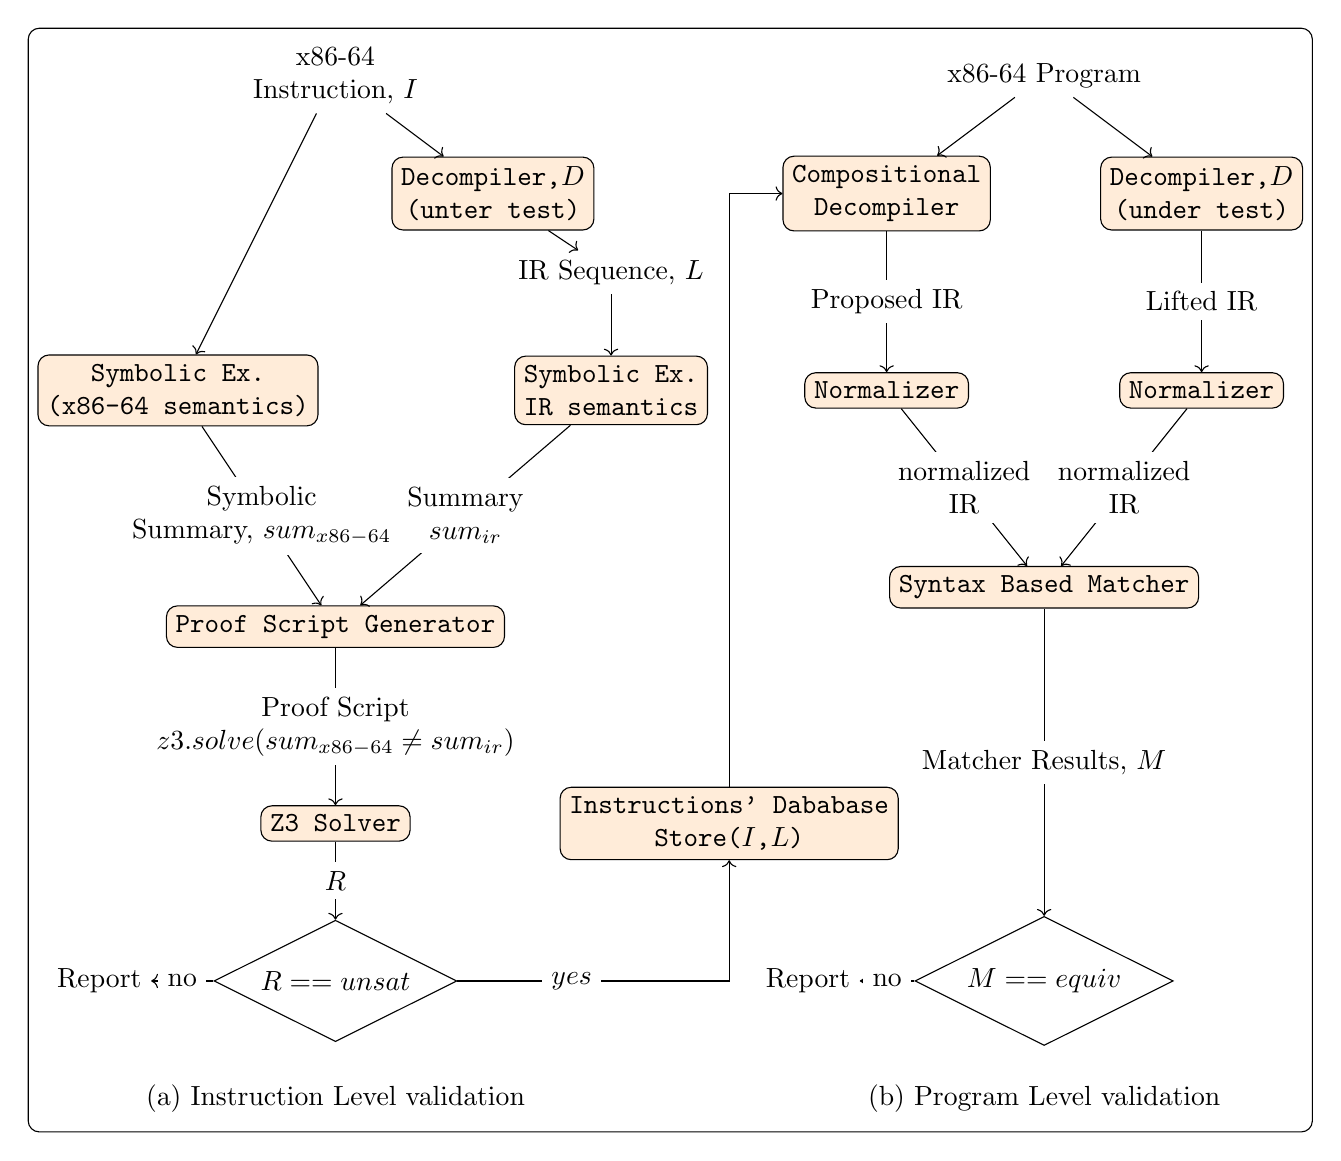
\begin{tikzpicture}[%node distance=2.5cm,
every node/.style={fill=white}, align=center]
\tikzset{%
    %>={Latex[width=2mm,length=2mm]},
    % Specifications for style of nodes:
    base/.style = {rectangle, rounded corners,
         text centered},
    process/.style = {base,  fill=orange!15, font=\ttfamily, draw=black},
    basic box/.style = {
        shape = rectangle,
        align = center,
        draw  = #1,
        %fill  = #1!25,
        rounded corners},
      header node/.style = {
        %Minimum Width = header nodes,
        font          = \strut\Large\ttfamily,
        text depth    = +0pt,
        fill          = white,
        draw},
      header/.style = {%
        inner ysep = +1.5em,
        append after command = {
            \pgfextra{\let\TikZlastnode\tikzlastnode}
            node [header node] (header-\TikZlastnode) at (\TikZlastnode.north) {#1}
            %node [span = (\TikZlastnode)(header-\TikZlastnode)] at (fit bounding box) (h-\TikZlastnode) {}
        }
      },
}
\def\blockhdist{2cm}
\def\blockvdist{1.5cm}
\def\phasehdist{8cm}


%%%%%%%%%%%%%%% PHASE I
\node (instr)          [base]  {\ISA\\ Instruction, $I$};
\node (SIVmcsema)   [process, below of=instr, yshift=-0.5cm, xshift=\blockhdist]  {Decompiler,$D$\\(unter test)};
\node (irseq)          [base,below of=SIVmcsema, xshift=\blockvdist]  {IR Sequence, $L$};
\node (instrSymEx)   [process, below of=instr, yshift=-2*\blockvdist, xshift=-\blockhdist] {Symbolic Ex.\\(\ISA semantics) };
\node (irSymEx)   [process, below of=irseq, yshift=-0.5cm] {Symbolic Ex.\\IR semantics};
\node (proofGen)   [process, below of=instr, yshift=-4*\blockvdist] {Proof Script Generator};
\node (solver)   [process, below of=proofGen, yshift=-\blockvdist] {Z3 Solver};
\node (decide1)     [draw, below of=solver, yshift=-1cm, diamond, aspect=2]  {$R == unsat$};
\node (report1)       [left of=decide1, xshift=-\phasehdist/4]  {Report};
\node (caption1)     [below of=solver, yshift=-2.5cm] {(a) Instruction Level validation};

\draw[->]             (instr) -- (SIVmcsema);
\draw[->]             (SIVmcsema) -- (irseq);
\draw[->]     (instr) -- (instrSymEx);
\draw[->]     (irseq) -- (irSymEx);
\draw[->]     (instrSymEx) -- node {Symbolic\\Summary, $sum_{\ISA}$} (proofGen);
\draw[->]     (irSymEx) -- node {Summary\\$sum_{ir}$ } (proofGen);
\draw[->]     (proofGen) -- node {Proof Script\\$z3.solve(sum_{\ISA} \ne sum_{ir})$} (solver);
\draw[->]     (solver.south) -- node {$R$} (decide1.north);
\draw[->]     (decide1.west) -- node {no} (report1);

%%%%%% Store
\node (store)     [process, right of=solver, xshift=\phasehdist/2]{Instructions' Dababase\\Store({$I$,$L$})};
\draw[->]       (decide1.east) -| node[xshift=-2cm] {$yes$} (store.south);


%%%%%%%%%%%% PHASE II
\node (start)             [base,right of=instr, xshift=\phasehdist]                       {\ISA Program};
\node (compd)             [process, below of=start, yshift=-0.5cm, xshift=-\blockhdist]          {Compositional\\Decompiler};
\node (mcsema)             [process, below of=start, yshift=-0.5cm, xshift=\blockhdist]          {Decompiler,$D$\\(under test)};
\node (normalizer1)             [process, below of=compd, yshift=-\blockvdist]   {Normalizer};
\node (normalizer2)         [process, below of=mcsema, yshift=-\blockvdist]   {Normalizer};
\node (matcher)     [process, below of=normalizer2, yshift=-\blockvdist, xshift=-\blockhdist]   {Syntax Based Matcher};
\node (decide2)     at (decide1 -| matcher) [draw,  diamond, aspect=2]  {$M == equiv$};
\node (caption2)     at (caption1 -| matcher) {(b) Program Level validation};
\node (report2)       [left of=decide2, xshift=-\phasehdist/4]  {Report};
 
 
\draw[->]             (start) -- (compd);
\draw[->]             (start) -- (mcsema);
\draw[->]     (compd) -- node {Proposed IR} (normalizer1);
\draw[->]     (mcsema) -- node {Lifted IR} (normalizer2);
\draw[->]     (normalizer1) -- node {normalized\\IR} (matcher);
\draw[->]     (normalizer2) -- node {normalized\\IR} (matcher);
\draw[->]     (matcher) -- node {Matcher Results, $M$} (decide2);
\draw[->]     (store.north) |-  (compd.west);
\draw[->]     (decide2.west) -- node {no} (report2);

%% Outter box
\begin{scope}[on background layer]
\node[fit = (compd)(mcsema)(start)(matcher), basic box = black,] (Phase1) {};
    \node[fit = (compd)(mcsema)(start)(matcher)(instr)(solver)(irseq)(instrSymEx)(irSymEx)(caption1)(caption2), basic box = black,] (Overview) {};
\end{scope}

\end{tikzpicture}


\end{figure*}



\section{Single \ISA Instruction Validation}
\section{Preliminaries}
\label{sec:Prelim}

Here we provide background on the \K framework and the \Strata project~\cite{Heule2016a} (used for our baseline semantics).

% briefly explain pieces of \ISA ISA necessary for our
% presentation. We also talk about \K, a semantics engineering tool which we
% chose to formalize our semantics into and  \Strata which gives us a head-start towards modeling the semantics of \ISA instructions.

%%% (VSA) DISABLE X86 BACKGROUND: IT IS WIDELY KNOWN
%\subsection{\ISA Instruction Set Architecture}

\ISA is the 64-bit extension of x86, a family of backward-compatible ISAs.
% x64 is a generic name for the 64-bit extensions to Intel's and AMD's 32-bit x86 instruction set architecture (ISA). 
%
We briefly explain some details of the architecture.

% Registers:
\ISA has the sixteen 64-bit general purpose registers (\reg{rax}--\reg{rdx}, \reg{rsi}, \reg{rdi}, \reg{rsp}, \reg{rbp}, \reg{r8}--\reg{r15}), and the two $64$-bit special registers (\reg{rip} and \reg{rflags}).
The lower $32$-, $16$- and $8$-bit portions of the register are referenced by the sub-register variants, e.g., \reg{eax}, \reg{ax}, and \reg{al} for \reg{rax}, respectively.
% \cmt{All these registers are used for storing integer values.}
The Haswell \ISA ISA additionally has sixteen 256-bit SIMD registers (\reg{ymm0}--\reg{ymm15}) along with the lower 128-bit sub-register variants (\reg{xmm0}--\reg{xmm15}).
% \cmt{, which are used for floating-point and packed operations.}

The \reg{rflags} register stores the current state of the processor.
Specifically, for example, the status flags such as the carry flag (\s{cf}), the parity flag (\s{pf}), the adjust flag (\s{af}), the zero flag (\s{zf}), and the sign flag (\s{sf}) are stored in \reg{rflags}.
These status flags are set according to the result of arithmetic and logical instructions.
% the status flags used mostly in user-level \ISA programs, and updated by arithmetic-logical instructions according to the result of the operation.
Some of control transfer instructions are performed based on the values of these flags.

% Addressing modes: 
\ISA supports the addressing modes, expressions that calculate a memory address to be read or written to. The addressing modes are used as the source or the destination of instructions that access the memory.
The addressing mode expressions can be generalized as:
$\s{base} + \s{index} \times \s{stride} + \s{offset}$.
In the assembly code, for example, \instr{-4(\reg{rax}, \reg{rbx}, 8)} denotes the address mode ``$\reg{rax} + \reg{rbx} \times 8 - 4$''.

% \cmt{      
% \begin{lstlisting}[style=SIMPRULES]
%     D (%RB, %RI, S)
%         RB is register for base
%         RI is register for index (0 if empty)
%         D is displacement (0 if empty)
%         S is scale 1, 2, 4 or 8 (1 if empty)
%     Effective Address: Mem[%RB + D + S*%RI]
% \end{lstlisting}
% }   

% Instruction variants:
% If an instruction access memory, we call it memory instruction. Else, if the instruction takes constant, then it is called immediate instruction. Otherwise, it is a register instructions.
\ISA has three types of instructions depending on the types of their operands: register instructions (with only register operands), memory instructions (with address mode operands), and immediate instructions (with constant operands).
The same mnemonic can be used for the different types of instructions.
For example, the mnemonic \instr{add} can be used for the register instructions (e.g., \instr{addq \reg{rax}, \reg{rbx}}\footnote{Throughout the presentation we will be using the {AT\&T} assembly syntax~\cite{Syntax} where the destination operand comes after source operands.}), the memory instructions (e.g., \instr{addq -4(\reg{rax}), \reg{rbx}}), and the immediate instructions (e.g., \instr{addq \$1, \reg{rbx}}).
% Throughout this paper, we will count each type of instructions as a different instruction.
% In the presentation, we will count them as different insructions ( and call them  instructions variants). Also different opcodes in the Intel manual are counted separately towards total instruction count. 
% \cmt{Whereas, register instructions differing on register names, immediate instructions differing on  constant values and memory instructions   differing on  memory addresses will be counted once towards total instruction count. }




\subsection{K Framework}\label{sec:KF}

%\K~\cite{k-primer-2013-v32} \cmt{\url{http://kframework.org}} is a framework for
%defining formal language semantics. Given a syntax and a semantics of a language, \K
%generates a parser, an interpreter, as well as formal analysis tools such as
%model checkers and deductive program verifiers, at no additional cost. Using
%the interpreter, one can test their semantics immediately, which significantly
%increases the efficiency of semantics developments. Furthermore, the formal
%analysis tools facilitate formal reasoning about the given language semantics.
%This helps both in terms of applicability of the semantics and in terms of
%engineering the semantics itself.
%
%We   refer the reader to~\cite{k-primer-2013-v32, rosu-serbanuta-2010-jlap} for
% details. In a nutshell, in \K, a language syntax is given using conventional
%Backus-Naur Form (BNF). A language semantics is given as a parametric
%transition system, specifically a set of reduction rules over configurations. A configuration is an algebraic representation of the
%program code and state. Intuitively, it is a tuple whose elements
%(called cells) are labeled and possibly nested. Each cell represents a
%semantic component, such as the memory or the registers. A special cell, named \s{k}, contains a
%list of computations to be executed. A computation is essentially
%a program fragment, while the original program is flattened into a
%sequence of computations. A rule describes a one-step transition
%between configurations, giving semantics to language
%constructs. Rules are modular; they mention only relevant cells that
%are needed in each rule, making many rules far more concise and easy to read
%than in some other formalisms.



% One of the most appealing aspects of K is its modularity. It is very rarely the
% case that one needs to touch existing rules in order to add a new feature to
% the language. This is achieved by structuring the configuration as nested cells
% and by requiring the language designer to mention only the cells that are
% needed in each rule, and only the needed portions of those cells. For example,
% the above rule only refers to the \s{k} and \s{regstate} cells, while
% the entire configuration contains many more cells (Figure
% ~\ref{fig:config}). This modularity makes for compact and human
% readable semantics, and also helps with the overall effectiveness of the
% semantics development. For example, even if new cells are later added to
% configuration, to support new features, the above rule does not change.

% \input{figures/configuration.tex}

\subsection{Strata Project}\label{sec:prelimstrata}
%% Support Count 
\Strata~\cite{Heule2016a} automatically synthesized formal semantics of \strataWithDupIS{} instruction variants (representing \strataIntel{} unique mnemonics) of the \ISA Haswell ISA. 
%% Set of test input 
The algorithm to learn the formal semantics of an instruction, say \s{IS}, starts with a small set of instructions, called base set \s{B}, whose semantics are known and trusted; a set of test inputs \s{T}, and the output behavior of \s{IS} obtained by executing \s{IS} on \s{T}. Then \Stoke~\cite{Stoke2013} is used  to synthesize  instruction sequences which contain instructions from \s{B} and match the behavior of \s{IS} for all test cases in \s{T}. Given two such generated instruction sequences \s{IS} and \s{IS}$^\prime$, their equivalence is decided  using an SMT solver and the trusted and known  semantics from the base set. If the two sequences are
semantically distinct, then the model produced by the SMT solver is used  to obtain
an input \s{t} that distinguishes \s{IS} and \s{IS}$^\prime$, and \s{t} is added to \s{T}. This process of synthesizing instruction sequence candidates and accepting or rejecting them based on equivalence checking with previous candidates, is repeated until a threshold is reached, which in their implementation is based on the number of accepted instruction sequences. 

%% Generalization 
\cmt{
Using the above technique, they first came up with the semantics of $692$ register
and $120$ immediate instructions. Then they used ``generalization'' of the register
instructions to get a total support count of \strataWithDupIS. Generalization is based on their hypothesis that the memory or immediate variants will behave identically with corresponding register variant (other than where the inputs come from) and hence can use the same formula as register variants. They validate this hypothesis using random testing. }

%% Two format of output
For each instruction, \Strata manifested its semantics in terms of two related artifacts.
The first artifact is an instruction sequence and the second is a set of SMT formulas 
in the bit-vector theory, one for each output register. 
The second is obtained by symbolically executing the first.

\cmt{
\Stoke~\cite{Stoke2013} contains manually written specifications  for a subset of the
x86-64 instruction set and there are APIs to generate SMT formulas from those specifications. 
\Strata uses those formulas to compare against the ones learned
by stratification by asking an SMT solver if the formulas are equivalent. For
example, for the instruction \instr{andnq \%rdx, \%rcx, \%rbx} the manually
written specification looks like the following:

\begin{lstlisting}[style=C++, label={lst:CS5}, caption={Manually Writen  specification for \instr{andnq
\%rdx, \%rcx, \%rbx}}]
semantic_function (
  Operand dst, Operand src1, Operand src2, 
  // dst == %rbx, src1 == %rcx, src2 == %rbx
  SymBitVector a, SymBitVector b, SymBitVector c, 
  // a, b, c are symbolic values for dst, src1, 
  // src2 resp. 
            SymState& ss) {
  // The symbolic state to be updated with the 
  // behaviour of the instruction     
  auto tmp = (!b) & c;
  
  // Setting destinaton
  ss.set(dst, tmp); 
  // Setting of, cf to false 
  ss.set(eflags_of, SymBool::_false()); 
  ss.set(eflags_cf, SymBool::_false());
  // Updating sf, zf based on result
  ss.set(eflags_sf, tmp[dst.size()-1]);
  ss.set(eflags_zf, tmp == SymBitVector::constant(dst.size(), 0));
  // Setting af, pf to undefined values
  ss.set(eflags_af, SymBool::tmp_var());
  ss.set(eflags_pf, SymBool::tmp_var());
}
\end{lstlisting}
}

\subsection{McSema}\label{sec:McS}



\section{\ISA Program-Level Validation}
\subsection{Compositional Decompiler}
\subsection{Normalizer}
\subsection{Matcher}

\chapter{Formal Semantics of \ISA User-Level ISA}\label{sec:results}
The equivalence checker being parametric on the semantics of source (\ISA) and target (LLVM) languages of decompilation, one of the important steps towards the goal is to define these semantics. In this section, we will discuss our published contribution~\cite{DasguptaAdve:PLDI19} is coming up with the most complete and thoroughly tested formal
semantics of x86-64 to date.


\section{Challenges in Formalizing \ISA}
\label{sec:challenges-in-formalizing-x86}
The \ISA instruction set architecture (ISA) is one of the most complex and widely used ISAs on servers and desktops, and ensuring the correctness of the \ISA binary code is important.
%
Completely formalizing the semantics of \ISA, however, is challenging especially due to the complexity and the sheer number of instructions that are informally specified in approximately 3,000-page standard~\cite{IntelManual}.
% In addition to the sheer number of instructions to be specified,
% % and the ambiguity of the informal standard document to consult,
% the following aspects make it challenging to completely specify the formal semantics of \ISA.

\paragraph{Size and Complexity:}
%
\SC{The \ISA ISA has a large number of instructions, partly because of a large number of complex instructions and partly because it keeps most of the legacy and deprecated instructions ($\sim$ \Xmmx{}+) for the sake of backwards compatibility.}
It consists of \totalIntel{} mnemonics, and each mnemonic admits several variants, depending on the types (i.e., register, memory, or constant) and the size (i.e., the bit-width) of operands.

\paragraph{Inconsistent Instruction Variants:}
%
Some variants have divergent behaviors more than the difference of their type and size. For example, \instr{movsd}, one of the 128-bit SSE instructions, has very different behaviors depending on whether the type of the source operand is register or memory; it clears the higher 64 bits of the target register only when the source type is memory.
Indeed, we revealed bugs in other semantics due to their incorrect generalization of the variants' behavior.

\paragraph{Ambiguous Documentation:}
%
The \ISA reference manual informally explains the instruction behaviors, leaving certain details unspecified or ambiguous, which required us to consult with an actual processor implementation to clarify such details.
%
Completely formalizing the vast number of instructions with carefully identifying all the corner cases from the informal document, thus, is highly non-trivial.


\paragraph{Undefined Behaviors:}
%
The \ISA standard also admits undefined behaviors that are implementation-dependent.
Many instructions (\undefIntel{}\footnote{\label{note1}These numbers are obtained by parsing the official manual ``Volume 2: Instruction Set Reference'' and cross checked with projects~\cite{Stoke2013, Felix} investing similar efforts.} out of \totalIntel{} mnemonics) have undefined behaviors: their output values of the destination register or the \reg{rflags} register are undefined in certain cases.
That is, the processor is free to choose any behavior in the undefined case.


Many existing semantics, however, simply ``define'' the undefined behaviors by
following a specific behavior taken by a processor implementation.
This approach is problematic because they do not capture all possible behaviors of different processor implementations.
Indeed, we found discrepancies between existing semantics in specifying the undefined behaviors, where different semantics are valid only for different groups of processors.
That is, such semantics are not adequate to formally reason about universal properties (e.g., portability) of a program that need to be satisfied for all standard-conforming processors.
%
For example, the parity flag \reg{pf} is undefined in the logical-and-not instruction \instr{andn}, where the processor implementation is allowed to either update the flag value (to 0 or 1), or keep the previous value.
We found, e.g., that Remill~\cite{Remill} updates the flag with 0, whereas Radare~\cite{Radare2} keeps it unmodified.
Identifying and faithfully specifying all the undefined behaviors, thus, are desirable but challenging.

\SC{In our semantics, we faithfully modeled the undefined value as a unique symbol (called \s{undef}) whose value is nondeterministically decided each time within the proper range.}
These nondeterministic values are enough to capture and formally reason about all possible behaviors of the instructions for different processors (and even any future, standard-conforming processor).

\section{Existing Semantics for \ISA}

To date, to the best of our knowledge, despite several explicit attempts~\cite{Heule2016a,Goel:FMCAD14,Goel:ProCoS17} and other related systems~\cite{Leroy:2009,Remill,TSL:TOPLAS13,Hasabnis:ASPLOS16,Hasabnis:FSE16},
no \emph{complete} formal semantics of \ISA exists that can be used for formal reasoning about x86 binary programs.
%
Heule~\etal \cite{Heule2016a} presented a formal semantics of \ISA, but it covers only a fragment ($\sim$\strataPerc{}) of all instructions; as the authors of \cite{Heule2016a} candidly admitted, their synthesis methodology proved insufficient to add the remaining instructions primarily due to limitations of the underlying synthesis engine. 
%
Moreover, their semantics misses certain essential details~\cite{DasguptaAdve:PLDI19}.
% and it has not been demonstrated how to use their semantics to formally reason about the functional correctness of the \ISA binary.\footnote{Although they provide a tool that can extract SMT formulae describing each instruction's behavior from their semantics, we found errors in their tool and thus the generated SMT formulae. Also, most of the SMT solvers are not designed to support rich reasoning principles.}
% natively support all the reasoning principles of the full-fledged proof assistants.}
% for the general purpose formal reasoning.}
%
% it is not clear how to lift their semantics to the full-fledged theorem prover to be able to reason about the full functional correctness of the \ISA binary.
% Although it can provide the semantics in the form of the SMT formulae, the SMT solver 
%
Goel~\etal~\cite{Goel:FMCAD14,Goel:ProCoS17}, on the other hand, specified a formal semantics in the \SC{ACL2} proof assistant~\cite{ACL2:Kaufmann2000}, allowing to reason about functional correctness, but their semantics covers only a small fragment ($\sim$\goelPerc{}) of all user-level instructions.
%\Comment{Section 2 says they had only 191 unique opcodes, which is only about 20\%, and even less if you include system instructions. Which is correct?}
%
There also have been several attempts~\cite{Angr1,BAP:CAV11,Radare2,Hasabnis:FSE16} to \emph{indirectly} describe the \ISA semantics, where they define an intermediate language (IL), specify the IL semantics, and translate \ISA to the IL.
This indirect semantics, however, may not be general enough to be used for different types of formal analyses, since the IL might be designed with specific purposes in mind, not to mention that the translation may miss certain important details of the instruction behaviors.
%
\section{Overview of the Approach}
\label{sec:Approach:Overview}

Briefly, our approach is as follows.
%
We first defined the machine configuration and underlying infrastructure in the \K framework, in order to define, execute and test the \ISA semantics.
%
\SC{To leverage previous work as much as possible, we took the semantic rules of all the instructions supported in Strata~\cite{Heule2016a}, which amounts to about 60\% of the instructions in scope, in the form of SMT formulas.}
%
We corrected, improved or simplified many of the baseline rules.
%
We then translated these SMT formulas from Strata into \K rules using a script, and tested the resulting rules by comparing with the Strata rules using Z3.
%
These steps give us a validated initial set of semantic rules in \K for about 60\% of the target instructions (our ``baseline'' set).

We attempted to extend the stratification approach in Strata to define additional rules automatically, in two ways: (i) augmenting their base set \s{B}, and (ii) constraining the search space manually using knowledge of instruction behaviors.  Both these attempts failed; they worked only for a few instructions, but in general, we found them to be impractical. Specifically, we added $58$ base instructions to the base set, and learned the semantics of $70$ new instructions, which are variants of the added  instructions, in $20$ minutes, but no more even after we kept running for two days. Also, we tried constraining the search space by manually populating it with relevant instructions. The lesson we learned from these experiments is, getting the right set of base instructions or a constrained search space for a complex instruction need an insight about the semantics of that instruction itself. We found that the effort to extract such information from the manual is about the same  as manually defining that instruction.


%\Comment{SANDEEP: Please check this last sentence and fix / improve.}

We then manually added \K rules for the remaining 40\% of the target instructions by systematically translating their description of the Intel manual into \K rules, in some cases cross-referencing against semantics available in Stoke.
%
The outcome was a complete formal specification of user-level \ISA in \K.

We validated this semantics in three ways:
%
First, we use the \K interpreter to execute the semantics of \emph{each} instruction for 7,000+ test inputs (each input is a processor state configuration) and compared the output directly with the hardware behavior for the same instruction.
%
Second, we repeated this experiment using the applicable programs in the \SC{GCC C-torture tests~\cite{CTORTURE}}.  % (\TortureInclude{} out of \TortureTotal{} tests).
%
Third, we compared against the semantics defined in the Stoke project for about 330 instructions that were omitted in Strata (thus not included in our baseline), using an SMT solver.

These validation experiments uncovered bugs~\cite{BugIntel,BugStoke983,BugStoke986} in the Intel manual, in Strata's simplification rules, and in the Stoke semantics.  All these bugs were reported to the respective authors, and most have been acknowledged and some have been fixed. Following is the brief summary of inconsistencies we found during the validation experiments.

\paragraph{Inconsistencies Found in the Intel Manual}
According to the manual, the semantics of \instr{vpsravd} \instr{\%xmm3,} \instr{\%xmm2,} \instr{\%xmm1} seems to depend on the lower $100$ bits of \reg{xmm3}, whereas the actual hardware execution suggests that it should depend on the lower $128$ bits. Similar inconsistencies are found in instructions with mnemonics \instr{vpsllvd}, \instr{vpsllvq}, \instr{vpsravd}.
Also, we found misleading typos related to instructions with opcodes \instr{vpsravw}, \instr{vpsravd}, \instr{vpsravq}, \instr{packsswb}.    
All these findings were reported and acknowledged by Intel as issues in the manual~\cite{BugIntel}.

\paragraph{Inconsistencies Found in \Strata's Simplification Rules}
While testing the instructions specifications borrowed from \Strata, we found inconsistent behaviors with the actual hardware. Moreover, the inconsistencies were discovered in the formulas of floating-point instructions. This is not surprising because \Strata models the floating-point instructions as \uif{} which cannot be executed or tested on hardware. Their semantics are executable in our definition though, and thus we were able to test them thoroughly. Note that Strata generates the formulas for these instructions by symbolically  executing  the corresponding learned  instruction sequences followed by a formula simplification pass. Therefore, errors in those formulas can be due to bugs either in the symbolic execution engine or in the simplification stage. Our testing shows that the second is true with the following evidence.
The simplification rule \s{add\_double(A, 0) == A} does not hold for \s{A = $-0.0$}. Same for \s{add\_single}. These were reported~\cite{PC1}.
Also, the simplification rule \s{sub\_double(A, A) == 0} does not hold for \s{A = $NaN$}.  Same is true for \s{sub\_single}. We found this bug in the  branch of Stoke which is used in \Strata. But this has been already fixed in the latest \Stoke branch.

\paragraph{Inconsistencies Found in \Stoke}

First, for instructions like \instr{addsubpd \%xmm1, \%xmm2} , the order of addition and subtraction specified by \Stoke is opposite to the one specified in the Intel Manual. Same is true with the mnemonic \instr{addsubps}. (Found in $12$ instruction variants.)

Second, the instruction \instr{pslld \%xmm1, \%xmm2} implements a logical left shift of packed data by a count specified in \reg{xmm1}. \Stoke's specification vectorized the operand \reg{xmm1} which is incorrect according to the manual. Similar issues were found in instructions implementing the logical right shift operations on packed data. (Found in  $18$ instructions.)

Third, \instr{cvtsi2sdl} \instr{\%eax,} \instr{\%xmm1} and \instr{vcvtsi2sdl} \instr{\%eax,} \instr{\%xmm0,} \instr{\%xmm1} are respectively SSE- and AVX-versions of the instruction to  convert a double-word ($32$-bit) integer to a scalar single-precision floating-point value. According to the manual, in the AVX-version,  the  destination bits $127-64$ of the  register \reg{xmm1} are updated to the corresponding bits in the first source operand \reg{xmm0}. This  is in contrast to the SSE-version of the instruction where the destination bits $127-64$ should remain unmodified. \Stoke specifies the semantics of the AVX-version similar to the SSE-version, which is incorrect.  (Found in $4$ instruction variants.)

Finally, some instructions, like \instr{imulb \%al}, which drive flag registers to an undefined state are not modeled correctly in \Stoke.    (found in $8$ instruction variants)

All these errors were reported and confirmed~\cite{BugStoke983,BugStoke986}.

\vspace{4pt}
Moreover, we illustrate the potential of our semantics to be used for formal analyses such as deductive program verification and program equivalence checking. For example, following are the three applications that we demonstrated:

\paragraph{Program Verification} To demonstrate that our semantics can be used to verify
x86-64 programs, we use the x86-64 verifier to prove the
functional correctness of the sum-to-n program. The functional correctness
property, which is $return-value = \sum_1^N n = N (N + 1) / {2}$ is specified as reachability specifications, essentially a pair of pre- and post-conditions for the function computing the sum-to-n.

\paragraph{Symbolic Execution to find Security Vulnerability}
\K automatically derives a correct-by-construction symbolic execution engine from the given semantics.
Being instantiated with our semantics, the engine can be used to symbolically execute and explore all possible paths in the given \ISA program.
We demonstrated how this capability can be used to find a  security vulnerability. We took a known security vulnerability using a code snippet of the HiStar~\cite{HiStar:2006} kernel. Using symbolic execution, we derive a path condition which can trigger the  vulnerability along with the triggering inputs.

\paragraph{Translation Validation of Optimizations}
\K also provides a program equivalence checker that can be used for the translation validation of compiler optimizations.
We derived an \ISA program equivalence checker from our semantics and used it to validate different optimizations of \s{popcnt} program which counts the number of set bits in the given input. We compiled the program with different optimizations: the GCC compiler optimizations (-O0, -O1, -O2, and -O3), and the Stoke super-optimization. We validated these optimizations by checking the equivalence between the optimized programs.


The \K framework also enables one to represent our semantics as SMT theories, which allows others to easily reuse our semantics for their own purposes.
\SC{%
    Indeed, we have translated our semantics to Stoke~\cite{completing-stock} which can serve as a drop-in replacement of Heule~\etal's semantics~\cite{Heule2016a} and can immediately benefit tools built on Stoke (e.g., \cite{Roessle:CPP19}).
}
%
% \paragraph{Artifacts}

Our formal semantics is publicly available at~\cite{x86-64-github}.



\chapter{Future Work}\label{sec:future}




%%%%%%%%%%%%%%%%%%%%%%%%%%%%%%%%%%%%%%%%%%%%%%%%%%%%%%%%%%%%%%%%%%%%%%%%%%%%%%%
% APPENDIX
%
\appendix
%\include{apx}

\backmatter

%%%%%%%%%%%%%%%%%%%%%%%%%%%%%%%%%%%%%%%%%%%%%%%%%%%%%%%%%%%%%%%%%%%%%%%%%%%%%%%
% BIBLIOGRAPHY
%

\bibliographystyle{IEEE_ECE}
% Put references in BibTeX format in thesisrefs.bib.
\bibliography{bibs/references.bib,bibs/modeling-X86-semantics.bib,bibs/bugs.bib,bibs/k.bib,bibs/decompilaion-validation.bib}
%\bibliography{thesisrefs}


%%%%%%%%%%%%%%%%%%%%%%%%%%%%%%%%%%%%%%%%%%%%%%%%%%%%%%%%%%%%%%%%%%%%%%%%%%%%%%%
% AUTHOR'S BIOGRAPHY
% As of 10/03/2011, Author's Biography or Vita no longer accepted by Grad College

\end{document}
\endinput
